% !TEX TS-program = pdflatex
% !TEX encoding = UTF-8 Unicode

% This is a simple template for a LaTeX document using the "article" class.
% See "book", "report", "letter" for other types of document.

\documentclass[10pt]{article} % use larger type; default would be 10pt

\usepackage[utf8]{inputenc} % set input encoding (not needed with XeLaTeX)

%%% Examples of Article customizations
	% These packages are optional, depending whether you want the features they provide.
	% See the LaTeX Companion or other references for full information.

%%% PAGE DIMENSIONS
\usepackage{geometry} % to change the page dimensions
	\geometry{letterpaper} % or letterpaper (US) or a5paper or....
	\geometry{margin=1in} % for example, change the margins to 2 inches all round
	% \geometry{landscape} % set up the page for landscape
	%   read geometry.pdf for detailed page layout information

\usepackage{graphicx} % support the \includegraphics command and options
\usepackage{caption}
\usepackage{subcaption}
\usepackage{sidecap}
%\usepackage{subcaption}

% \usepackage[parfill]{parskip} % Activate to begin paragraphs with an empty line rather than an indent

%%% PACKAGES
\usepackage{booktabs} % for much better looking tables
\usepackage{array} % for better arrays (eg matrices) in maths
\usepackage{paralist} % very flexible & customisable lists (eg. enumerate/itemize, etc.)
\usepackage{verbatim} % adds environment for commenting out blocks of text & for better verbatim
% \usepackage{subfig} % make it possible to include more than one captioned figure/table in a single float
%\usepackage{datetime} %suggested to get todays data and time
% These packages are all incorporated in the memoir class to one degree or another...

\usepackage{listings} % For displaying code

\usepackage{placeins}      % This package gives us \FloatBarrier

\usepackage{mathtools} % this will also load amsmath package

%%% HEADERS & FOOTERS
\usepackage{fancyhdr} % This should be set AFTER setting up the page geometry
\pagestyle{fancy} % options: empty , plain , fancy
\renewcommand{\headrulewidth}{0pt} % customise the layout...
\lhead{}\chead{DSCI 351-351M-451 Syllabus: Exploratory Data Science}\rhead{}
%\lfoot{}\cfoot{\thepage}\rfoot{}
\lfoot{\today}\cfoot{}\rfoot{\thepage}

%%% SECTION TITLE APPEARANCE
\usepackage{sectsty}
\allsectionsfont{\sffamily\mdseries\upshape} % (See the fntguide.pdf for font help)
% (This matches ConTeXt defaults)

%\usepackage[labelfont = footnotesize, textfont = small, justification=centering]{caption}  %allows us to change the font of the captions on figures
%\setlength{\abovecaptionskip}{5pt}
%\setlength{\belowcaptionskip}{-10pt}

\usepackage{wrapfig}  %allows figures to have text wrapped around them. Apparently this does not work perfectly in Latex and requires manual adjustment of figures and such

\hyphenation{op-tical net-works semi-conduc-tor}
%
%\usepackage{parskip}
%\setlength{\parindent}{5pt}

\usepackage{enumitem}  %%%%allows you to begin enumerate at 0

%%%Allows you to have \textsubscript as a command
%\usepackage{fixltx2e}

\usepackage{longtable}

%%% ToC (table of contents) APPEARANCE
\usepackage[nottoc,notlof,notlot]{tocbibind} % Put the bibliography in the ToC
\usepackage[titles,subfigure]{tocloft} % Alter the style of the Table of Contents
\renewcommand{\cftsecfont}{\rmfamily\mdseries\upshape}
\renewcommand{\cftsecpagefont}{\rmfamily\mdseries\upshape} % No bold!

\newcommand{\squeezeup}{\vspace{-2.5mm}}

%%%must be the last package called
\usepackage{hyperref}
\hypersetup{colorlinks=true, linkcolor=blue, citecolor=blue, filecolor=blue, urlcolor=blue, pdftitle=DSCI351-351M-451, pdfauthor=RHF, pdfsubject=DSCI351-351M-451, pdfkeywords=DSCI351/351M/451}

%%% END Article customizations

%%% The "real" document content comes below...

\title{DSCI 351-351M-451 Syllabus \\ \emph{Exploratory Data Science} \\ Fall 2022 	Tuesday, Thursday 11:30 am to 12:45 pm NORD 356 \& Remote/Synchronous}
\author{Prof. Roger H. French (CWRU), \\ Prof. Laura S. Bruckman (CWRU), \\ Prof. Paul Leu (Pitt), \\ Prof. Kris Davis (UCF), \\ Prof. Sonya Cirlos (UTRGV)}
%\date{} % Activate to display a given date or no date (if empty),
         % otherwise the current date is printed

\begin{document}
\maketitle

%\begin{figure} [!htbp]
%\centering
%	\includegraphics[height=.4\textheight]{figs/1501DSCI351Syllabus}
%	\caption{Syllabus, concepts and organization}
%	\label{fig:Syllabus}
%\end{figure}

%-------------------------------------------------------

\tableofcontents

%-------------------------------------------------------

\section{Joint Undergraduate and Graduate Course}

  \subsection{Case Western Reserve University (CWRU): DSCI351 and DSCI351M}

    DSCI351 is the 3rd level class in the Applied Data Science Undergraduate Minor.
    The ADS Minor is available to CWRU students across all the schools in the University.
    For more information see Applied Data Science Undergraduate Minor in the CWRU Bulletin \href{https://bulletin.case.edu/engineering/materials-science-engineering/applied-data-science-minor/}{Undergraduate minor in Applied Data Science}.

    DSCI351 will introduce students to the basic elements of a data analysis, including R coding, Rstudio IDE and Git version control, statistical concepts, the stages of a data analysis and reproducible research.

    DSCI351M section focuses specifically on Exploratory Data Science for Materials and Materials' Systems.

  \subsection{Case Western Reserve University (CWRU): DSCI451}

    DSCI 451 is a graduate level introduction to data science and analytics.
    DSCI 451 is one of the classes that satisfy the University Graduate Certificate in Applied Data Science.
    For more information on the University Graduate Certificate in Applied Data Science, see  \href{https://bulletin.case.edu/engineering/materials-science-engineering/applied-data-science-graduate-certificate/}{Grad. Cert. in Applied Data Science} that is now available to students in all CWRU Schools and Colleges.
    Graduate students will develop a semester long data science project focused on time-series, spectral, image, statistical process control or machine learning data science problems that are relevant to their research interests.
    These projects will include preparing datasets, code scripts and functions, a git repository for other students to use these codes as open source resources, and the preparation of reproducible data science analyses for these problems.

    \begin{figure}[htbp]
      \centering
      \begin{subfigure}{0.3\linewidth}
        \centering
        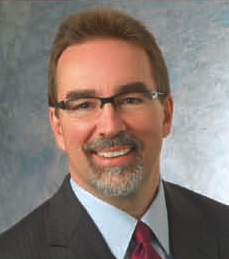
\includegraphics[width=0.5\textwidth]{figs/roger_french.jpg}
        \caption{CWRU Prof. Roger French.}
        \label{fig:french}
      \end{subfigure}
      \hfill
      \begin{subfigure}{0.3\linewidth}
        \centering
        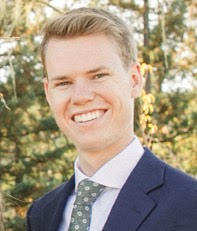
\includegraphics[width=0.5\textwidth]{figs/WillOltjen.jpg}
        \caption{CWRU TA: Will Oltjen}
        \label{fig:oltjen}
      \end{subfigure}
        \begin{subfigure}{0.3\linewidth}
        \centering
        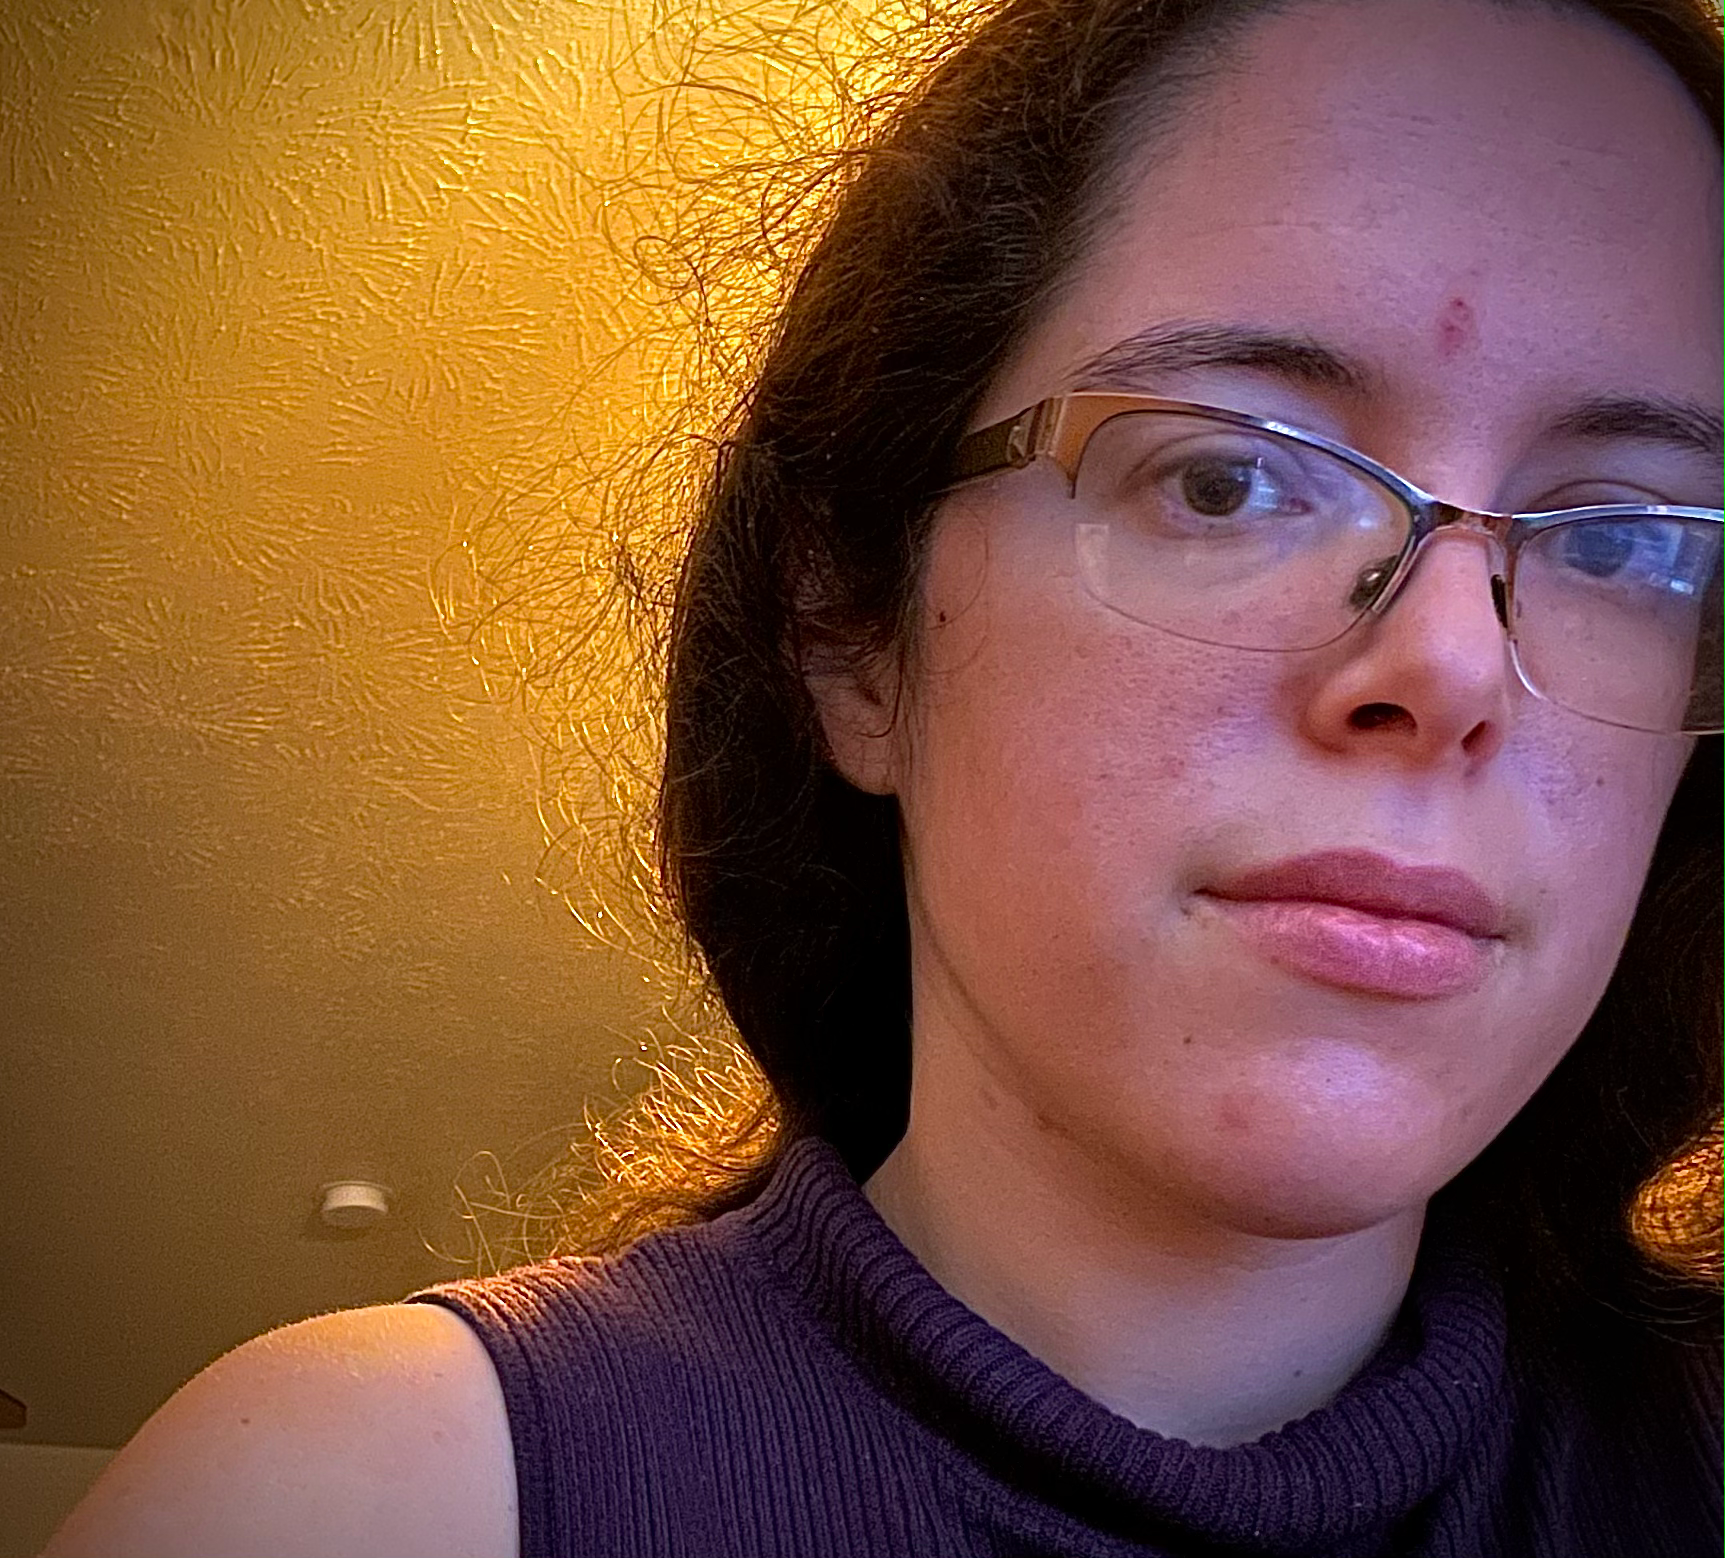
\includegraphics[width=0.5\textwidth]{figs/KristenHernandez.png}
        \caption{CWRU TA: Kristen Hernandez}
        \label{fig:kristen}
      \end{subfigure}
      \caption{The CWRU Team.}
      \label{fig:cwru}
    \end{figure}

  \subsection{Univ. of Pittsburgh (Pitt): ENGR 1451 and ENGR 2451}

    As part of a research collaboration between CWRU and Pitt, where we have established the \href{https://www.mds-rely.org}{NSF IUCRC Center for Materials Data Science for Reliability and Degradation}, this year we are co-teaching the UG and GS DSCI 351/451 and DSCI 353/453 classes so that students at Pitt will learn data science with us this semester.  The Pitt students will submit their Lab Exercises and Exams to the Pitt Canvas site for ENGR 1451/2451, and these will be graded independently of the CWRU students.

    \begin{figure}[htbp]
      \centering
      \begin{subfigure}{0.3\linewidth}
        \centering
        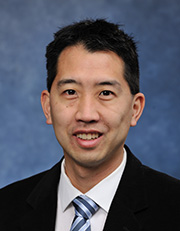
\includegraphics[width=0.5\textwidth]{figs/PaulLeu.jpg}
        \caption{UCF Prof. Paul Leu.}
        \label{fig:paul}
      \end{subfigure}
      \hfill
      \begin{subfigure}{0.3\linewidth}
        \centering
        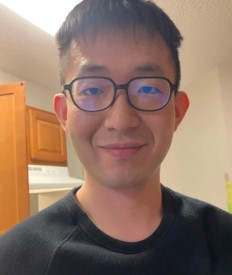
\includegraphics[width=0.5\textwidth]{figs/MingxuanLi.jpeg}
        \caption{UCF TA: Mingxuan Li}
        \label{fig:mingxuan}
      \end{subfigure}
      \caption{The Pitt Team. }
      \label{fig:Pitt}
    \end{figure}

  \subsection{Univ. of Central Florida (UCF): EMA 6908}

    As part of a research collaborations between CWRU and UCF, we have studied photovoltaics and reliability of technologies under real-world exposure conditions.  We are co-teaching the UG and GS DSCI 351/451 and DSCI 353/453 classes so that students at UCF will also be able to learn data science with us this semester. The UCF students will submit their Lab Exercises and Exams to the UCF Canvas site for EMA 6908, and these will be graded independently of the CWRU students.

    \begin{figure}[htbp]
      \centering
      \begin{subfigure}{0.3\linewidth}
        \centering
        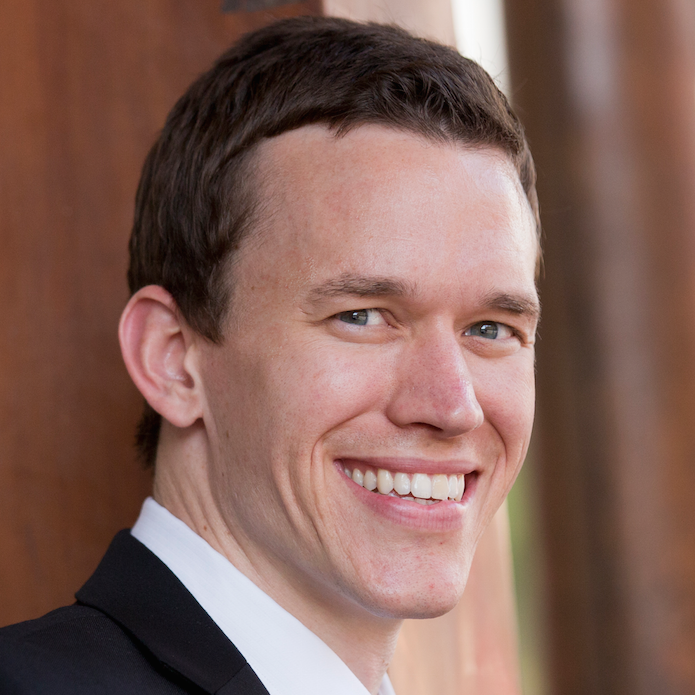
\includegraphics[width=0.5\textwidth]{figs/Kris_Davis.png}
        \caption{UCF Prof. Kris Davis.}
        \label{fig:davis}
      \end{subfigure}
      \hfill
      \begin{subfigure}{0.3\linewidth}
        \centering
        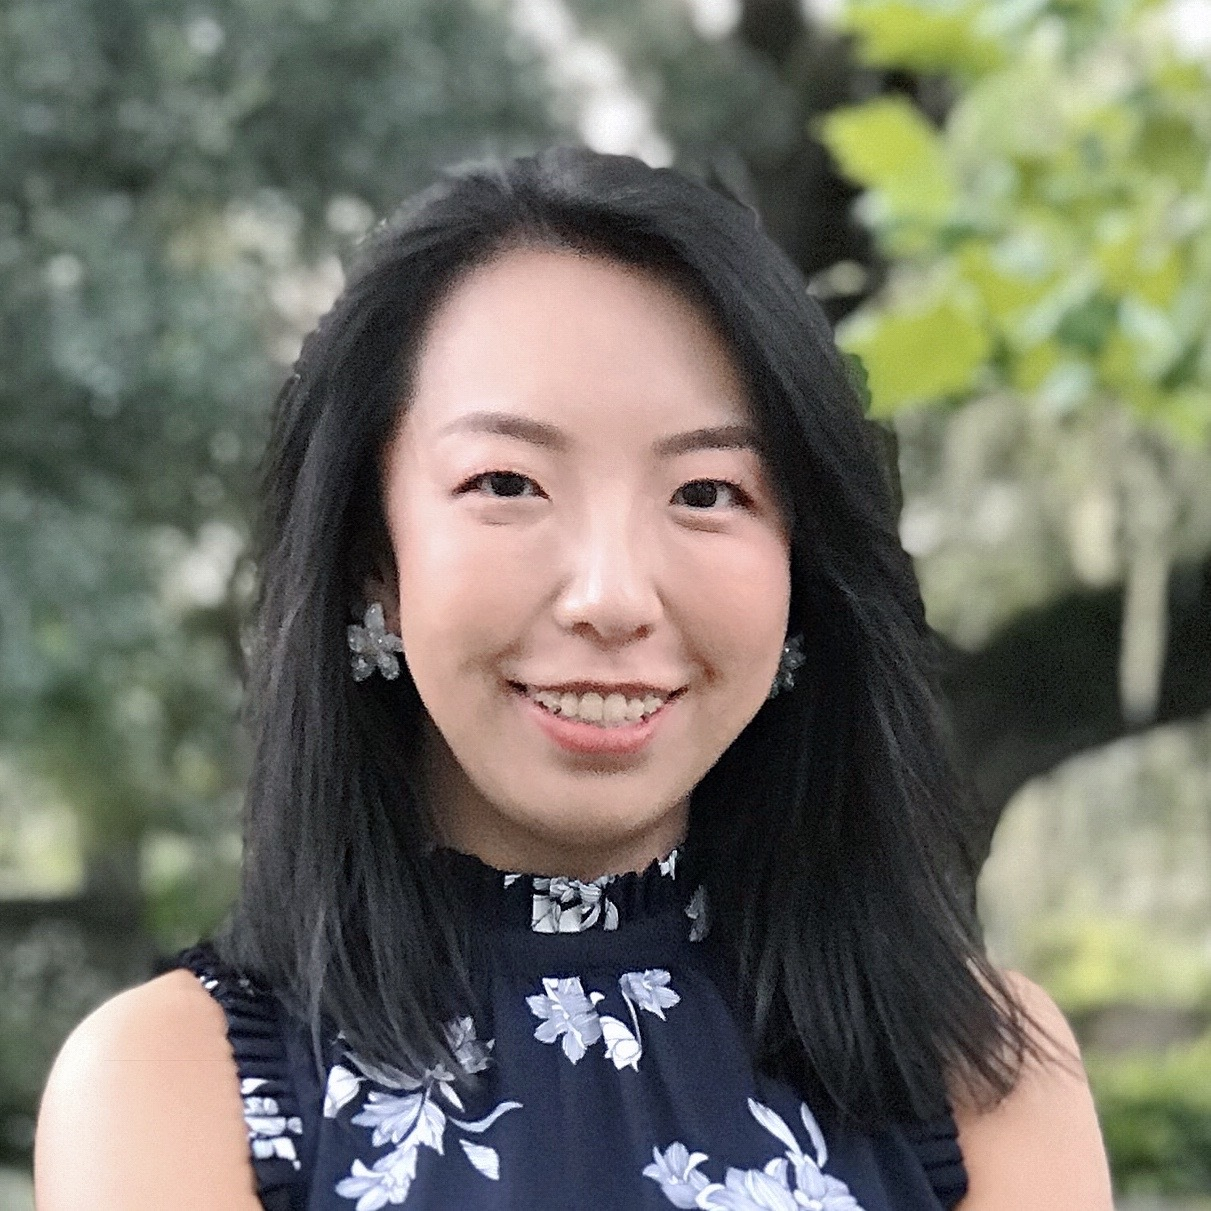
\includegraphics[width=0.5\textwidth]{figs/Mengjie_Li.jpg}
        \caption{UCF TA: Mengjie Li}
        \label{fig:mengjie}
      \end{subfigure}
      \begin{subfigure}{0.3\linewidth}
        \centering
        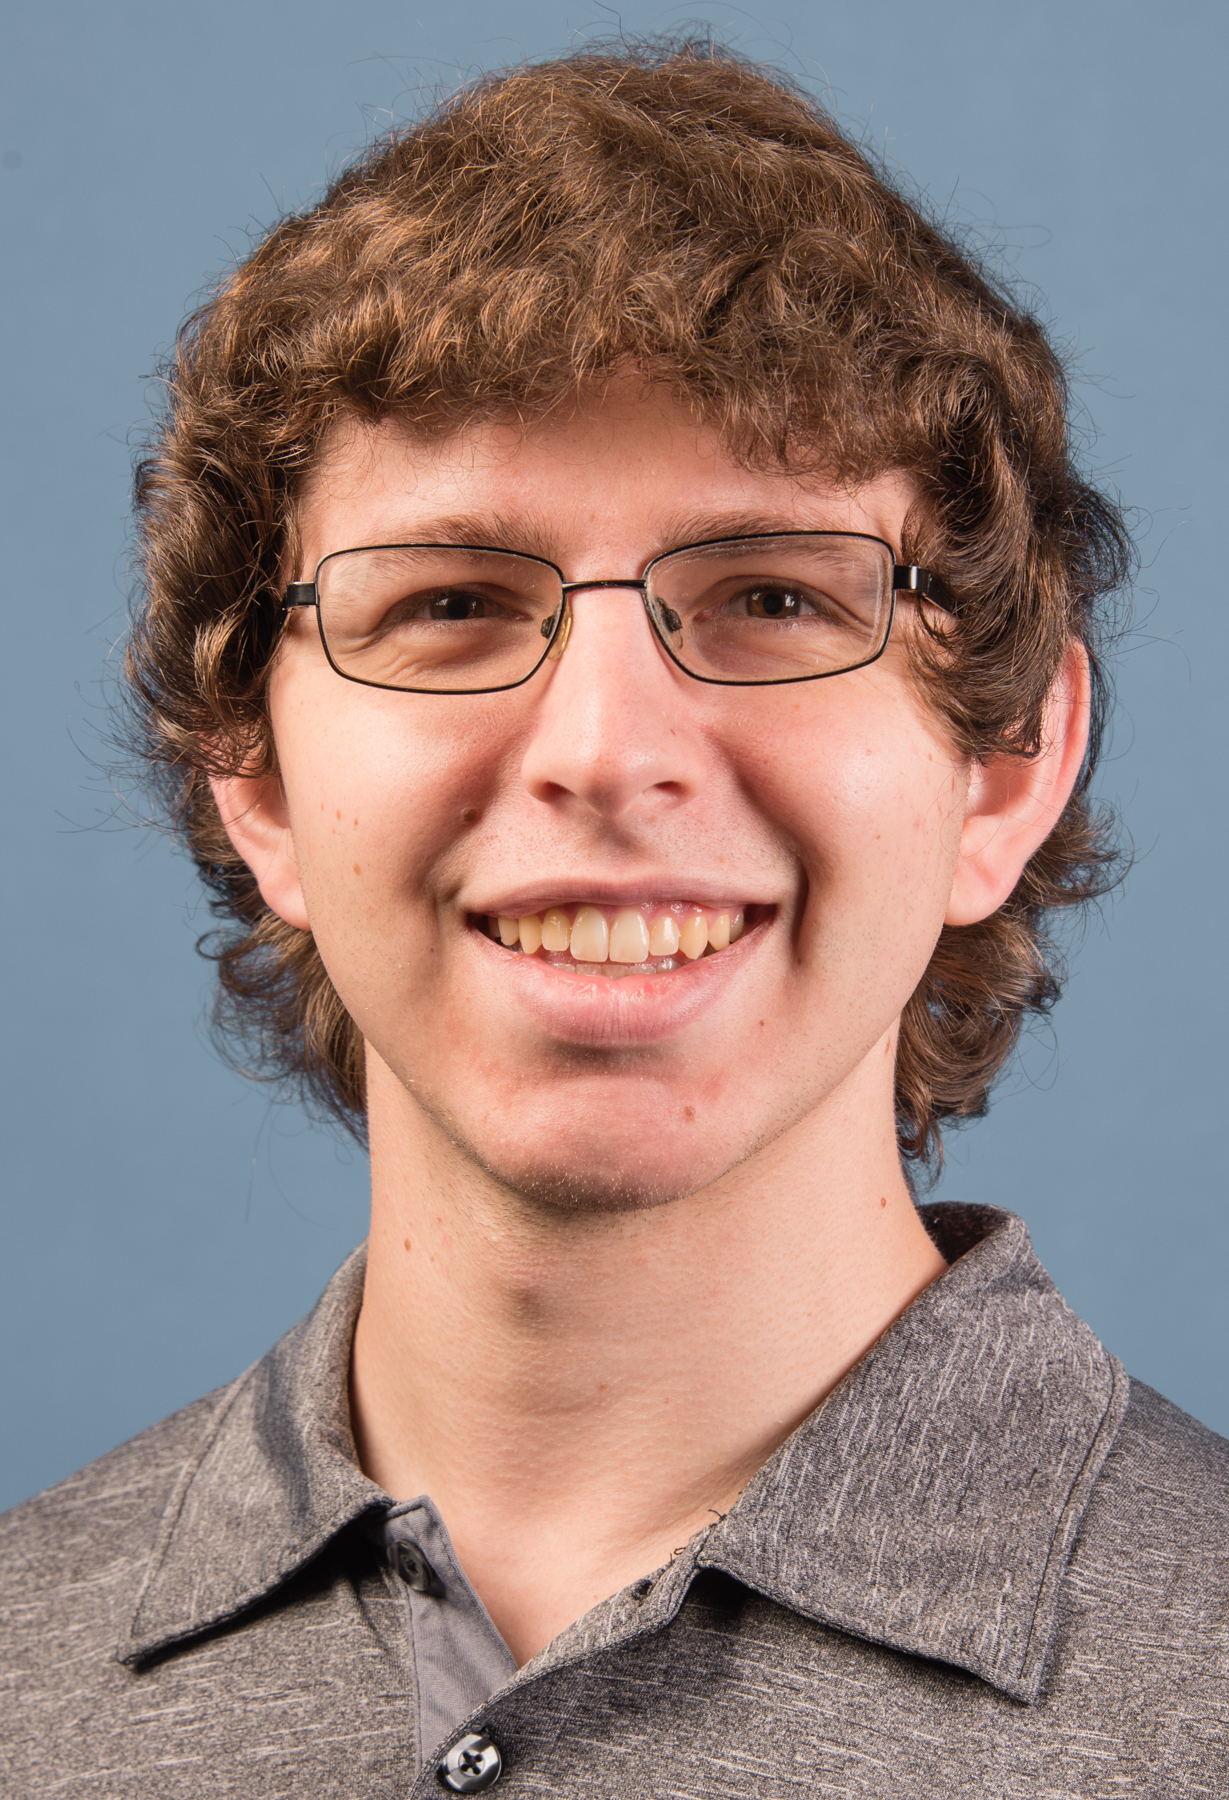
\includegraphics[width=0.5\textwidth]{figs/Dylan_Colvin.jpg}
        \caption{UCF TA: Dylan Colvin}
        \label{fig:dylan}
      \end{subfigure}
      \caption{The UCF Team.}
      \label{fig:UCF}
    \end{figure}

  \subsection{Univ. of Texas, Rio Grande Valley (UTRGV): CSCI 4341-04}

    As part of ongoing collaborations between CWRU and UCF, we are co-teaching the UG and GS DSCI 351/451 and DSCI 353/453 classes so that students at UTRGV will also be able to learn data science with us this semester. The UTRGV students will submit their Lab Exercises and Exams to the UTRGV Canvas site for CSCI 4341-04, and these will be graded independently of the CWRU students.

    \begin{figure}[htbp]
      \centering
      \begin{subfigure}{0.3\linewidth}
        \centering
        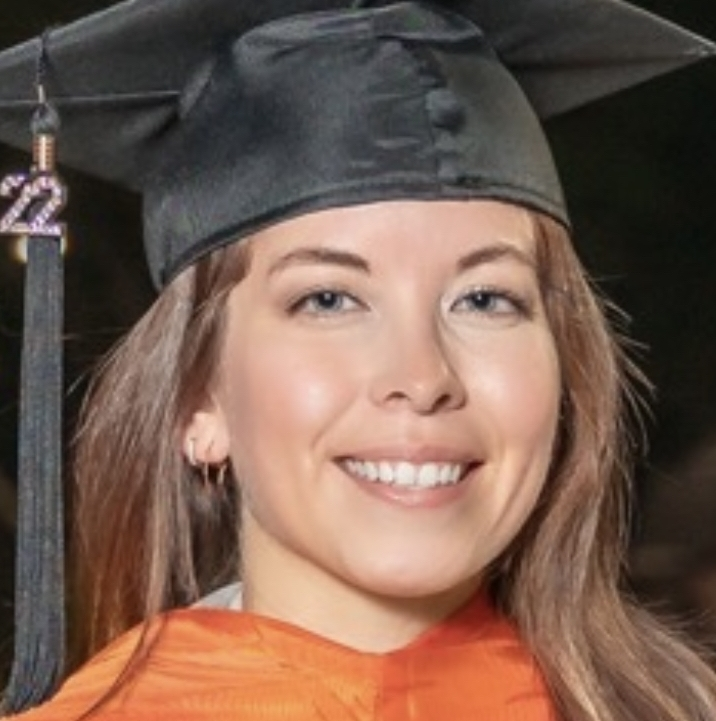
\includegraphics[width=0.5\textwidth]{figs/SonyaCirlos-crop.jpeg}
        \caption{UTRGV Prof. Sonya Cirlos}
        \label{fig:sonya}
      \end{subfigure}
      \hfill
      \begin{subfigure}{0.3\linewidth}
        \centering
        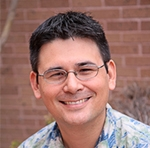
\includegraphics[width=0.5\textwidth]{figs/emmett-tomai-cr.jpg}
        \caption{UTRGV Prof. Emmett Tomai}
        \label{fig:emmett}
      \end{subfigure}
      \caption{The UTRGV Team. }
      \label{fig:UTRGV}
    \end{figure}

    So lets welcome our Pitt, UCF and UTRGV partners!



\section{Course Description}

  In this course, we will learn data science and analysis approaches to identify statistically significant relationships and better model and predict the behavior of these systems.
  We will assembly and explore real-world datasets, perform clustering and pair-wise correlation plot analyses to investigate predictor/variable correlations, and linear and logistic regression will be employed to develop associated predictive models.
  Results will be interpreted, visualized and discussed.

  We will introduce basic elements of statistical analysis using the R coding language (\href{"http://cran.case.edu/"}{R Project open source software}) for exploratory data analysis and model development.
  R is an open-source software project with broad abilities to access machine-readable open-data resources, data cleaning and munging functions, and a rich selection of statistical packages, used for data analytics, model development and prediction.
  This will include an introduction to R data types, reading and writing data, looping, plotting and regular expressions, so that one can start performing variable transformations for linear fitting and developing structural equation models, while exploring for statistically significant relationships.
  We will also learn tidy principles for data analysis, pipes and ggplot vs base graphics approaches to data visualization.
  Python is also commonly used for data science and data analyses, while at the same time Python is a general purpose programming language.  Both R and Python are interpreted languages that do not require compiling the code prior to execution.
  Due to Python's broader spread of use cases (from data analysis to full applications to software engineering) it can be easier for a developing data scientist to find useful answers to questions, by learning R first.
  Python can then be learned as a second data analysis language.
  Students are welcome to use Python in the DSCI classes.

  R Analytics will be applied to the case of time-series, spectral, image problems using continuous and categorical variables and  datasets to analyze system responses, combined with results of experiments to identify fundamental principles that are statistically significant in the observed system performance.
  We will learn about longitudinal and cross-sectional data science studies, along with retrospective and prospective studies.

  The class is taught using a ``practicum'' approach and will be structured to have a balance of theory and practice.
  We'll split class into Foundation and Practicum
    a) Foundation: lectures, presentations, discussion
    b) Practicum: coding, demonstrations and hands-on data science work.

  Every student will have access to their own pre-configured Open Data Science Desktop computer, already configured for fast and easy adoption of good data science practices and tools.
  And the ODS VDIs are updated each month so as to have the latest versions of R packages and software for data science.
  And also introduces students to doing applied data science and data analysis on both Windows or Macintosh notebook computers, and also in Linux based High Performance Computing environment, using Markov, CWRU's data science cluster.

  \subsection{Class Repository Folder Structure}

    Please browse within each folder to learn more about the intended purpose of each folder in the standard structure.

    This folder structure has been designed to accommodate each type of file you may need to create and modify - please do not create additional folders in the structure, and please pay attention to naming conventions when creating new files.

    Course Material Folders in this Course Repository
    \begin{itemize}
      \item 1-Assignments is where you will find the Lab Exercises and Exams
      \item 2-Readings folder contains textbooks and readings for the course
      \item 3-Class contains daily class notes as *.Rmd and *.pdf files
      \item These are split into a Foundations "f" and a Practicum "p" class notes
      \item 4-Syllabus contains the updated Course Syllabus
      \item 5-SemProj contains the materials needed for DSCI451
    \end{itemize}

    Your Working Data Analysis Folders
    \begin{itemize}
      \item Scripts is where to write you scripts for data analysis
      \item Data contains course datasets and your datasets
      \item Figs is the figures folder, accessible for both Scripts, Topics and Docs
      \item Topics is where to write reports and presentation for your data analysis
      \item Docs is where to write formal documentation as *.Rmd, *.tex files
      \item Packages is where to build R packages, if your project involves this
    \end{itemize}

  \subsection{License applied to course materials and some datasets used for data analysis}

    Class materials
    \begin{itemize}
      \item License: This work is legally bound by the following software license: [CC-A-NS-SA-4.0][1]
      \item Please see the LICENSE.txt file, in the root of this repository, for further details.
    \end{itemize}

    Assessment materials
    \begin{itemize}
      \item Lab Exercise Assignments, Project Assignments and Exams are all rights reserved.
      \item They are NOT creative commons licensed, and can not be distributed.
    \end{itemize}

    Datasets derived from funded research projects
    \begin{itemize}
      \item During this class you may be working on a project that is part of a funded research award at Case Western Reserve University.
      \item Information or material made available to you in connection with this funded research project, and coursework, data, results or other intellectual property you may develop in conjunction with this project, will be subject to Case Western Reserve’s Intellectual Property Policy as well as terms of the sponsored research agreement.
      \item You acknowledge that you understand that you will not have ownership of intellectual property created in conjunction with the project.
      \item Please sign the ``2208-DSCI-Acknowledgement-of-IP.pdf'' form. And email it to Jonathan Steirer at \href{mailto:jws227@case.edu}{jws227@case.edu}
    \end{itemize}

  \subsection{Outcomes}

    {\bf Capabilities}
    \begin{itemize}
    	\item Familiarity with R Statistics, scripting, functions, packages, automated data analysis.
    	\item Familiarity with exploratory data analysis, statistical model building.
        \item Familiarity with Principles of Tidy Data Science from the tidyverse package an use of pipes ( $\%>\%$ ) from the magrittr package.
    	\item Applications of domain knowledge and statistical analytics to identify important predictors and develop initial predictive models.
    	\item Applications of domain knowledge and analytics to identify important predictors and develop initial predictive models.
    	\item Introduction to methods of reproducible research, including markdown, LaTeX and Git.
    \end{itemize}

    {\bf Data types include:}
    \begin{itemize}
    	\item Time-series, spectral, image and higher order datatypes,
    	\subitem And their assembly to produce augmented and derivative datasets.
    \end{itemize}

    {\bf Data set characteristics will include:}
    \begin{itemize}
    	\item Variety: Types of data and information, including both structured and unstructured data.
    	\item Volume: Data from human sources (vendors, suppliers, distributors, customers, etc.) and sensor networks,  both small and large data volumes.
    	\item Velocity: Short time interval datasets.
    \end{itemize}

  \subsection{Prerequisites}

    \begin{enumerate}
      \item ENGR131 Elementary Computer Programming, EECS132, or equivalent
      \item STAT312R Basic Statistics for Engineering and Science or equivalent
    \end{enumerate}

\section{Textbooks and Readings}

  Required Texts and their Abbreviation, which is used in the syllabus:

  Peng R Programming (PRP) and Peng Exploratory Data Analysis (EDA) are introductory books to R and Data Science and Analysis.
  These are  LeanPub books, available from LeanPub for a ”pay what you want” price.

  R for Data Science (R4DS) is a new book teaching R for Tidy Data Science, and is available as a bookdown book on the web \href{http://r4ds.had.co.nz/}{R for Data Science}, you can buy an ebook for \$18 from \href{https://play.google.com/store/books/details/Hadley_Wickham_R_for_Data_Science?id=I6y3DQAAQBAJ}{Google Play Store page for this book}.

  Open Intro Statistics version 4 (OIS) is an open source text book on Inferential Statistics, published under a Creative Commons license, \href{https://drive.google.com/file/d/0B-DHaDEbiOGkc1RycUtIcUtIelE/view}{for free distribution as a pdf}.
  In addition a copy can be purchased from Amazon for \$20.

  Introduction to Statistical Learning with R, 2nd Edition (ISLR) was just released this year and is a \href{https://link.springer.com/book/10.1007/978-1-0716-1418-1}{Springer} book which is also available for  \href{https://www.statlearning.com/}{free as a pdf}. ISLR is the text book used extensively in DSCI353/453 on Statistical and Machine Learning.

  %\FloatBarrier

  \begin{SCfigure}
  	\centering
  	\caption{{\bf PRP}: Roger Peng, {\bf \textsc{R Programming for Data Science}}. 2014 \cite{peng_r_2014}}
  	\includegraphics[width=0.2\textwidth]%
  	{figs/Peng-R-Programming.png}% picture filename
  \end{SCfigure}

  \begin{SCfigure}
  	\centering
  	\caption{{\bf EDA}: Roger Peng, {\bf Exploratory Data Analysis With R}. 2015 \cite{peng_exploratory_2015}}
  	\includegraphics[width=0.2\textwidth]%
  	{figs/Peng-EDAwithR.png} % picture filename
  \end{SCfigure}

  \begin{SCfigure}
  	\centering
  	\caption{{\bf OIS}: David M. Diez, Christopher D. Barr, and Mine Cetinkaya-Rundel, \href{"https://www.openintro.org/stat/textbook.php"}{ {\bf OpenIntro Statistics 4th Ed.} } 2015 \cite{david_m._diez_openintro_2015} }
  	\includegraphics[width=0.2\textwidth]%
  	{figs/OISv4.jpg} % picture filename
  \end{SCfigure}

  \begin{SCfigure}
      \centering
      \caption{{\bf R4DS}: Garrett Grolemund, Hadley Wickham {\bf R for Data Science}. 2017 \cite{wickham_r_2017}}
      \includegraphics[width=0.2\textwidth]%
      {figs/r4ds.png}% picture filename
  \end{SCfigure}

  \begin{SCfigure}
  	\centering
  	\caption{ {\bf ISLR}: Gareth James, Daniela Witten, Trevor Hastie, Robert Tibshirani {\bf An Introduction to Statistical Learning: with Applications in R, 2nd Edition}, 2021  \cite{james_introduction_2013} }
  	\includegraphics[width=0.2\textwidth]%
  	{figs/ISLR-2ndEd.jpg} % picture filename
  \end{SCfigure}

  Additional reading assignments will be distributed via the course git repository in the readings subdirectory.

%-------------------------------------------------------

\section{Grading: Lab Exer., SemProj Rep. \& Pres., MidTerm \& Final Exam}

{\bf DSCI351 and DSCI351M is graded on 100 points basis}
\begin{align*}
  Seven \, Lab \ Exercise \ (LE) \ Data \, Analyses, \\
  LE1,LE2 \ = 7 \ points \ each, \ = \ 14 \ pts.\\
  LE3-LE7 \ worth \, 10 \, points \, each \ = \ 50 \ pts.\\
  Three \, SemProject \ Report \ Presentation \ Evaluations \ (2 pt/each) = 6 \ pts. \\
  Midterm \, Exam = 10 \ pts.\\
  Final \, Exam = 20 \ pts. \\
  {\bf Total = 100 \ pts}
\end{align*}

{\bf DSCI451 is graded on a 140 point basis}
\begin{align*}
  Seven \, Lab \ Exercise \ (LE) \ Data \, Analyses, \\
  LE1,LE2 \ = 7 \ points \ each, \ = \ 14 \ pts.\\
  LE3-LE7 \ worth \, 10 \, points \, each \ = \ 50 \ pts.\\
  Midterm \, Exam \ = \ 10 \ pts.\\
  Final \, Exam \ = \ 20 \ pts. \\
  Three \, Report \ Presentation \ Evaluations \ (2 pt/each)  = \ 6 \ pts. \\
  Six \, SemProj \, Updates \, worth \, (2 \, point \, each) \, =  \ 12 \ pts. \\
  One \, SemProj \, with \,3 \, presentations (5 pts/each) \, \& \,1 \, Final \, Report (13 pts) = \ 28 \ pts. \\
  {\bf Total = 140 pts}
\end{align*}


Grading is done on a curve.

All Lab Exercise assignments are submitted electronically through Canvas, uploading to the LE assignment page. by Midnight on the day they are due.

Late submission of Lab Exercises will result in loss of 1 point for each day they are late.

More details about grading are in the Course Mechanics section of the syllabus.


\FloatBarrier
\section{DSCI351-351M-451 Syllabus: Weekly Topics}
\begin{table}[h]
  \centering % used for centering table
  \begin{tabular}{| p{2.9cm} | p{3.9cm} | p{3.9cm} | p{1.8
        cm} | p{2.5cm} |} % centered columns (5 columns)
	\hline %inserts horizontal line
	{\bf Day:Date} & {\bf Foundation} & {\bf Practicum} & {\bf Reading} & {\bf Due} \\ % inserts table heading
	\hline
	\hline % inserts double horizontal line
%	 w01\addtolength{}{•}
  w01a:Tu:8/30/22 & ODS Tool Chain & R, Rstudio, Git & & \\ % inserting body of the table
	\hline %inserts single line
	w01b:Th:9/1/22 & Setup ODS Tool Chain & Bash, Git, Slack, Agile & PRP4-33 & LE1 \\
	\hline
	\hline
	w02a:Tu:9/6/22 & Bash-Git-Knuth-Lit.Prog. & RIntroR & PRP35-64  &  \\
	\hline
	w02b:Th:9/8/22 & What is Data Science & OIS:Intro2R & OIS1,2 &  \\
	\hline
	w02Pr:Fr:9/9/22 &  & & PRP65-93 & {\bf 451 Update1} \\
	\hline
	\hline
	w03a:Tu:9/13/22 & Data Intro & Data Analytic Style & PRP94-116 & LE2 {\bf LE1 Due} \\
	\hline
	w03b:Th:9/15/22 & Rand. Var. Normal Dist. & Git, Rmds, Loops & OIS4 &  \\
	\hline
	\hline
	w04a:Tu:9/20/22 & Tidy Check Explore  & Tidy GapMinder & EDA1-31 &  \\
	\hline
	w04b:Th:9/22/22 & Inference, DSCI Process & Other Distrib. 7 ways & R4DS1-3 & LE3 {\bf LE2 Due} \\
	\hline
	w04Pr:Fr:9/23/22 & & & EDA32-58 & {\bf 451 Update2} \\
	\hline
	\hline
	w05a:Tu:9/27/22 & OIS4 Rand. Var. & EDA of PET Degr. & OIS5 &  \\
	\hline
	w05b:Th:9/29/22 & OIS5 Found. of Infer. & Multivar Corr. Plot & R4DS4-6 & \\
	\hline
	w05Pr:Fr:9/30/22 &  & & & {\bf 451 RepOut1} \\
	\hline
	\hline
	w06a:Tu:10/4/22 & Pred., Algorithm, Model &   & R4DS7-8 &  \\
	\hline
	w06b:Th:10/6/22 &  Summ. Stats \& Vis. & Anscombe's Quartets &  R4DS9-16 & LE4 {\bf LE3 Due} \\
	\hline
	w06Pr:Fr:10/7/22 &  &  & & {\bf 451 Update3} \\
	\hline
	\hline
	w07a:Tu:10/11/22 & Midterm Rev. Tidy Data & Correl Plots Summ Stats  & OIS6.1-2 & {\bf PeerRv1 Due} \\
	\hline
	w07b:Th:10/13/22 & HypoTest, Infer. Recap & Penguin EDA, Sampling &  &  \\
	\hline
	\hline
	w08a:Tu:10/18/22 & {\bf MIDTERM}  &  {\bf EXAM}  &  \\
	\hline
	w08b:Th:10/20/22 & Programming \& Coding  & Code Packaging  &  & {\bf LE4 Due} \\

		\hline
	w08Pr:Fr:10/21/22 & & & & {\bf 451 Update4} \\
	\hline
	\hline
	Tu:10/24,25 &  {\bf CWRU} & {\bf FALL BREAK} & R4DS17-21 \\
%  w09a:Tu:10/19/22 & 1 Prop. \& Dif. of 2 Prop.  & Cat. Inf. & R4DS17-21 & \\
	\hline
	w09b:Th:10/27/22 & Cat. Inf. 1 \& 2 propor. & Indep. Test,2-way tables & OIS6.3-4  & LE5  \\
	\hline
	w09Pr:Fr:10/28/22 &  & & & {\bf 451 RepOut2} \\
	\hline
	\hline
	w10a:Tu:11/1/22 & Goodness of Fit, $\chi^2$ test & t-tests 1\&2 means & OIS7.1-4 &  \\
	\hline
	w10b:Th:11/3/22 & Num. Infer, Cont. Tables & Stat. Power  &  &  \\
	\hline
	w10Pr:Fr:11/4/22 & & & & {\bf 451 Update5} \\
	\hline
	\hline
	w11a:Tu:11/8/22 & Sample \& Effect Size & Stat. Power GGmap  & OIS8 & {\bf PeerRv2 Due} \\
	\hline
	w11b:Th:11/10/22 & Regr Part 1, Test \& Train & Curse of Dimen. & ISLR1,2.1,2 & LE6 {\bf LE5 Due} \\
	\hline
	\hline
	w12a:Tu:11/15/22 & Regr. Outliers & Regr Part 2, GIS & OIS9 &  \\
	\hline
	w12b:Th:11/17/22 & Mult.Regr., Var. Select & Regr. Diagnostics &  \\
	\hline
	w12Pr:Fr:11/18/22 & & & & {\bf 451 Update6} \\
	\hline
	\hline
	w13a:Tu:11/22/22 & Log. Regr. & Mult. Regression & ISLR3.1 & LE7 {\bf LE6 due} \\
	\hline
	w13b:Th:11/24/22 & Statistical learning & Logistic Regr. & ISLR3.2 &  \\
  \hline
  w13Pr:Fr:11/25/22 & & & & {\bf 451 RepOut3} \\
	\hline
	\hline
	w14a:Tu:11/23/22 &  & GIS Trends & ISLR4.1-3 &  \\
  \hline
  Th,Fr:11/24,25 & {\bf THANKSGIVIING} & {\bf Vacation} & \\
	\hline
	\hline
	w15a:Tu:11/29/22 & Classificat., Sup. Lrning & Log. Regr. \& ML & & {\bf PeerRv3 Due}  \\
  \hline
  w15b:Th:12/1/22 & Clustering, Unsup. Lrning & Caret, Broom 4 modeling & Fr.Br.2020 &   \\
	\hline
	w15SPr:Fr:12/2/22 &  &  &   &  \\
	\hline
	\hline
  w16a:Tu:12/6/22 & Big Data Analytics & Dist. Comp., Hadoop & Khalil.2020 &   \\
  \hline
  w16b:Th:12/8/22 & Final Exam Review &  & Mirletz,2015 & {\bf LE7 due}  \\
  \hline
  \hline
  {\bf Friday 12/12} & {\bf SemProj} & {\bf Final Report}  & & {\bf SemProj4 due} \\
	\hline
	{\bf Monday 12/19} & {\bf FINAL EXAM} &  {\bf 12:00-3:00pm} & Nord 356 & or remote  \\
	\hline
	\hline
  \end{tabular}

  \caption{DSCI351-451 Weekly Syllabus. w01a is week 1, class a. w01b is week 1 class b. w02Pr is DSCI451 SemProj. Readings are defined by book and chapters, sections in Peng R Prog. (PRPx.y), Peng Exp. Data An. (EDAx.y), R for Data Sci. (R4DSx.y), Open Intro Stats (OISx.y) \& Intro. to Stat. Learn. with R (ISLRx.y).}
  \label{table:Syllabus} % is used to refer this table in the text
\end{table}

\FloatBarrier

%-------------------------------------------------------
\section{Contact Information}

  Prof. Roger H. French
  \begin{itemize}
  	\item White 536, and electronically.
  	\item Email is best: rxf131@case.edu, Use DSCI351 in the subject line
  	\item @frenchrh on twitter
  	\item Office Phone 216 368 3655, Cell Phone 302 468 6667
  \end{itemize}

DSCI 351-351M TA: Will Oltjen
  \begin{itemize}
    \item White 614, and electronically.
    \item Email is best: wco3@case.edu, Use DSCI351-451 in the subject line
    \item @WillOltjen on twitter
    %\item Lab Phone 216 368 0135, %Cell Phone: (216) 303-0733
  \end{itemize}

DSCI 351-351M TA: Kristen Hernandez
  \begin{itemize}
    \item White 615, and electronically.
    \item Email is best: kjh125@case.edu, Use DSCI351-451 in the subject line
    %\item @ on twitter
    %\item Lab Phone 216 368 0135, %Cell Phone: (216) 303-0733
  \end{itemize}

-------------------------

  DSCI 451 Prof. Laura S. Bruckman
  \begin{itemize}
    \item White 502A, and electronically.
    \item Email is best: lsh41@case.edu, Use DSCI351 in the subject line
    \item @bruckman\_laura on twitter
    %\item Office Phone 216 368 3655, Cell Phone 302 468 6667
  \end{itemize}

  DSCI 451 TA: Nat Tomczak
  \begin{itemize}
  	\item White 615, and electronically.
  	\item Email is best: nkt8@case.edu, Use DSCI351-451 in the subject line
  	%\item @liu\_jiqi on twitter
  	%\item Lab Phone 216 368 0135, %Cell Phone: (216) 303-0733
  \end{itemize}

-------------------------

  ENGR 1451-2451 Pitt Prof: Paul Leu
\begin{itemize}
  \item electronically.
  \item Email is best: pleu@pitt.edu, Use ENGR 1451-2451 in the subject line
  \item @Paul\_W\_Leu on twitter
  % \item Lab Phone 216 368 0135, %Cell Phone: (216) 303-0733
\end{itemize}

  ENGR 1451-2451 Pitt TA: Mingxuan Li
\begin{itemize}
  \item electronically.
  \item Email is best: MIL152@pitt.edu or mxl1261@case.edu, Use ENGR 1451-2451 in the subject line
  %\item @liu\_jiqi on twitter
  % \item Lab Phone 216 368 0135, %Cell Phone: (216) 303-0733
\end{itemize}

-------------------------

  EMA 6908 UCF Prof: Kris Davis
    \begin{itemize}
      \item electronically.
      \item Email is best: kristopher.davis@ucf.edu, Use EMA 6908 in the subject line
      \item @kris\_o\_davis on twitter
      % \item Lab Phone 216 368 0135, %Cell Phone: (216) 303-0733
    \end{itemize}

  EMA 6908 UCF TA: Mengjie Li
    \begin{itemize}
      \item electronically.
      \item Email is best: menglie.li@ucf.edu, Use EMA 6908 in the subject line
      %\item @ on twitter
      % \item Lab Phone 216 368 0135, %Cell Phone: (216) 303-0733
    \end{itemize}

  EMA 6908 UCF Prof: Dylan Colvin
    \begin{itemize}
      \item electronically.
      \item Email is best: kristopher.davis@ucf.edu, Use EMA 6908 in the subject line
      \item @kris\_o\_davis on twitter
      % \item Lab Phone 216 368 0135, %Cell Phone: (216) 303-0733
    \end{itemize}

-------------------------

  CSCI 4341-04 Prof: Sonya Cirlos
\begin{itemize}
  \item electronically.
  \item Email is best: sonya.cirlos01@utrgv.edu, Use CSCI 4341-04 in the subject line
  \item @CirlosSonya on twitter
  % \item Lab Phone 216 368 0135, %Cell Phone: (216) 303-0733
\end{itemize}


%-------------------------------------------------------
\section{Course Mechanics}

  \subsection{Lectures}

    Fall 2012 	Tuesday, Thursday 11:30 am to 12:45 pm, Nord 356 and Remote/Synchronous on Zoom

  \subsection{Consultations}

    Office hours are Monday and Wednesday from 4pm to 5pm on Zoom, invites in the Canvas Course Calendar.

    Lab Exercise questions and solutions can be discussed in Office Hours or in the class Slack Channel.

    After class or as needed. Contact Prof. French or the TAs, by Slack, email.

  \subsection{Lab Exercise Assignments}

    All Lab Exercise assignments are submitted electronically through Canvas, uploading to the LE assignment page. by Midnight on the day they are due.

    Late submission of Lab Exercises will result in loss of 1 point for each day they are late.


    Filenames should contain DSCI351, -LE\#, -YourLastName... e.g. DSCI351-LE2-French.R or DSCI351-LE2-French.R and DSCI351-LE2-French.pdf.

    Lab Exercises need to be legible, organized and explain your thinking, process and results.
    Credit all resources you drew upon, including texts, papers, peers.

    Lab Exercises are due prior to class on the day they are due.

    Lab Exercises will be graded on canvas and reviewed in class.

    Lab Exercise solutions will be reviewed in Office Hours

  \subsection{451 Semester Project Template}

    Students in DSCI 451 and ENGR 2451 have a 40 point semester-long data science project to do.

    Prof. Laura Bruckman and TA Raymond Wieser organize and consult on the semester projects.

    Please see the projectreport-template.Rmd for the template for 451 Updates and Report Outs
    Report Outs can be presented as the projectreport-template or as an .Rpres presentation



  \subsection{CWRU Data Science Slack}

    We have a CWRU Data Science Slack

    You can join by signing up at \href{https://cwru-dsci.slack.com}{https://cwru-dsci.slack.com}

    Sign up using your case.edu email address

    There is a specific class channel, along with general, applied data science and job opportunities channels.

    The class Slack channel is a good place for discussing questions from class and/or assignments.

%-------------------------------------------------------

\section{Coding and Data Science Tools and Resources}

  {\bf Markov Data Science Cluster} \\

    You will not need to install software on your personal computers.

    We have a High Performance Computing Cluster dedicated to Data Science courses.

    It is named Markov after \href{https://en.wikipedia.org/wiki/Andrey_Markov}{Andrey Markov}. .

    To access Markov, sign in to the OnDemand website using your caseID, \href{https://ondemand.case.edu}{https://ondemand.case.edu}

    There you will see the an icon for the OnDemand Apps.

    The ``RStudio Server R/4.1.1, Shared by Roger French (rxf131)'' is what we will use for class.

    As a back up, you will also see ``RStudio Server R/3.6.3, Shared by Roger French (rxf131)'' which is using the prior version of the R programming language.

    It can be useful to login using the Firefox or Vivaldi browswers, since OnDemand wants you to quit your browser at the end of a session. \\


  {\bf Open Data Science (ODS) Win10 Desktops} \\

    You will not need to install software on your personal computers.

    Instead you can login to the CWRU My Apps portal. \cite{cse_portal_cwru_2014}

    The CWRU MyApps portal is located at \href{https://myapps.case.edu}{https://myapps.case.edu}

    How to access your ODS Desktop from a computer

    The \href{new MyApps portal}{https://myapps.case.edu},
    allows us to better scale back-end processing as necessary based on load.

    All apps and student files have been migrated.

    There will be more public announcements of MyApps in the coming weeks, but we wanted to make sure that you had the information now.

    You can access your ODS Desktop, from any modern Browser (Chrome, Firefox).

    Or you can install the Citrix Workspace Client program on you computer

    -----


    \begin{itemize}
      \item     Documentation is included below.

      \item \href{https://drive.google.com/open?id=1FXUoD_p-pMnoPTO7DPsDSVFr9t8vQmp8y-7xxdvvIfw}{''MyApps Streamed Applications and Desktops - Usage Manual''}

      \item Windows, Linux

      \item \href{https://drive.google.com/open?id=1__lS_43YQ1-6exw0EsP3RKnOT3AJKAtR5oqLleT590g}{MyApps Citrix Workspace Setup (Windows)}

      \item \href{https://drive.google.com/open?id=1rzVb7ZFDjRVfc8Zjtn_F8jqbxD67gtDrvSnqUhVeQyI}{Reset Citrix Workspace App on Windows}

      \item macOS:

      \item \href{https://drive.google.com/open?id=1v2O91Zf4rmSo2Qoxq_l3JVQNPaFPrllSDxZB8CYSnz8}{MyApps Citrix Workspace Setup (macOS)}

      \item \href{https://drive.google.com/open?id=1rzVb7ZFDjRVfc8Zjtn_F8jqbxD67gtDrvSnqUhVeQyI}{Reset Citrix Workspace App on macOS}
    \end{itemize}


    -----

    If there are any issues accessing MyApps, please call the HelpDesk (368-HELP, \href{mailto:help@case.edu}{help@case.edu} to submit a ticket, and CSE-IT team will assist.

    -----

    {\bf Scripting, Coding and Writing} \\
    And more resources for open science coding and scripting, including tools for code editing, code version control and languages.

    {\bf R Statistics} \\
    We will be using R in this class for Lab Exercises and SemProjs.
    Its generally useful language for statistical analysis and data science.

      \begin{itemize}
        \item \href{"http://www.r-project.org/index.html"}{The R Project for Statistical Computing}  \cite{r_r_2014} main website
        \item \href{"http://en.wikipedia.org/wiki/R_(programming_language)"}{R programming language}  R is a free software programming language and software environment for statistical computing and graphics.\cite{r_project_r_2014}
        \item \href{"http://www.rstudio.com/"}{ RStudio} provides popular open source and enterprise-ready professional software for the R statistical computing environment. \cite{rstudio_rstudio_2014}
        \item \href{"https://google-styleguide.googlecode.com/svn/trunk/Rguide.xml"}{ Google's R Style Guide}
      \end{itemize}

    {\bf Rmarkdown} as a path to open access and reproducible science

      \begin{itemize}
        \item \href{"http://rmarkdown.rstudio.com/"}{ R Markdown — Dynamic Documents for R.} We will be doing all our work using Rmarkdown this semester.
        Class presentations, Lab Exercises, semester projects, all done in Rmd, as reproducible science projects, including data, code, and final output.
        \item \href{"http://shiny.rstudio.com/articles/rmarkdown.html"}{ Introduction to R Markdown.}
        \item \href{"http://www.rstudio.com/resources/cheatsheets/"}{ R Markdown Cheat Sheets.}
        \item \href{"http://rpubs.com/mansun_kuo/24330"}{ An Rmarkdown Introduction slidedeck done from Rmarkdown and shared publicly on RPubs.}
      \end{itemize}

    {\bf R Statistics, more resources} \\
       We will be using R in this class for lab exercises and projects. Its generally useful language for statistical analysis and data science.
      \begin{itemize}
        \item \href{"http://www.r-project.org/index.html"}{The R Project for Statistical Computing}  \cite{r_r_2014} main website
        \item \href{"https://www.youtube.com/user/rdpeng/playlists"}{Roger Peng's Computing for Data Analysis introduction to R Statistics}.
        These are from a \href{"https://www.coursera.org/course/compdata"} {Coursera course} he does, with the same name. \cite{peng_computing_2014}\item \href{"http://cran.r-project.org/doc/contrib/Torfs+Brauer-Short-R-Intro.pdf"}{A (very) short introduction to R}  \cite{torfs_very_2014}
        \item \href{"https://google-styleguide.googlecode.com/svn/trunk/Rguide.xml"}{ Google's R Style Guide}
        \item \href{"http://stat405.had.co.nz/r-style.html"}{ Hadley Wickham's R Style Guide}
        \item \href{"http://www.rstudio.com/resources/cheatsheets/"}{ RStudio's R Cheatsheets for Rmarkdown and Data Wrangling}
        \item \href{"http://www.theresearchkitchen.com/blog"}{An Rmd slideshow Intro to R}
      \end{itemize}

    {\bf Open Source software and tools} \\

      \begin{itemize}
        \item \href{"http://en.wikipedia.org/wiki/Portal:Free_software"}{FOSS (Free and Open Source Software)} is a copyleft approach to software which is hat is distributed in a manner that allows its users to run the software for any purpose, to redistribute copies of, and to examine, study, and modify, the source code. \cite{_portal:free_2014}
        \item \href{"http://www.vim.org/"}{vim (or Gvim the gui version)} is a powerful text and code editor, that is universally available on all linux and mac computers.\cite{_gvim_2014}   \href{"http://neovim.org/"}{NeoVim} is a new Gvim fork.\cite{_neovim_2014} It can be installed on windows computers, its available on the ODS Desktops.. \cite{_gvim_2014}
        \item \href{"http://en.wikipedia.org/wiki/Git_(software)"}{Git (Wikipedia)} is a distributed content versioning system that is very popular. It enables collaborative code development and LaTeX writing projects.\cite{_git_2014-2}
        \item \href{"http://git-scm.com/"}{Git server software} is installed on each computer.\cite{_git_2014}
        \item  \href{"https://github.com/"}{GitHub} is a Git server website used for collaborative code development.\cite{_github_2014}
        \item  \href{"https://bitbucket.org/"}{BitBucket} is a Git server website used for collaborative code development. If you join with your case.edu email address, you get unlimited private repositories.\cite{_bitbucket:_2014}
        \item \href{"http://stackexchange.com/tour"}{Stack Exchange}  \cite{stack_exchange_stack_2014} Code Question and Answer Websites: covering R, Python, Mathematica, {LaTeX} and many other things, such as English or Spanish etc.
      \end{itemize}

    {\bf Python3 (is also used for Data Science in many cases. But here we will focus on R first. }

      \begin{itemize}
        \item \href{"https://en.wikipedia.org/wiki/Python_(programming_language)"}{Wikipedia: Python is a widely used general-purpose, high-level programming language.}  \cite{python_python_2014}
        \item \href{"https://www.python.org/"}{The Python main website.} \cite{python_python.org_2013}
        \item \href{"https://docs.python.org/3/tutorial/index.html"}{The Python Tutorial — Python v3.8.5 documentation}  \cite{python_python_2014}
        \item \href{"http://docs.python-guide.org/en/latest/"}{The Hitchhikers Guide to Python}. This is an open access book being hosted on developed on \href{"https://github.com/"}{GitHub} and is located here \href{"https://github.com/vuvlab/python-guide"}{https://github.com/vuvlab/python-guide}. \cite{_hitchhikers_2014} \cite{_kennethreitz/python-guide_2014}
        \item \href{"http://www.numpy.org"}{NumPy is the fundamental package} \cite{numpy_numpy_2014} for scientific computing with Python.
        \item \href{"http://www.ctcms.nist.gov/fipy/"}{FiPy: Partial Differential Equations with Python} \cite{guyer_fipy:_2009}
        \item \href{"http://www.scipy.org/"}{SciPy is a python-based ecosystem}  \cite{scipy_scipy.org_2014} of open-source software for mathematics, science, and engineering.
        \item \href{"http://ipython.org/index.html"}{IPython Shell and Notebook}  \cite{ipython_ipython_2014}
        \item \href{"https://code.google.com/p/spyderlib/"}{Spyder is the Scientific Python Development Environment}  \cite{spyder_spyder_2014}
      \end{itemize}

    {\bf LaTeX is used for publication quality writing. Its also the backend for Rmarkdown's pdf generation. It lets you write professional looking papers, theses and books, along with presentations. }
      \begin{itemize}
        \item \href{"http://www.tug.org/"}{LaTeX} is a program for writing documents, paper, journal articles, presentations and theses. \cite{_tex_2014}
        \item \href{"http://en.wikibooks.org/wiki/LaTeX"}{LaTeX - Wikibooks}, open books for an open world. \cite{latex_latex_2014}
        \item \href{"https://www.zotero.org/"}{Zotero Reference-Citation Manager, BibTeX Client}  \cite{zotero_zotero_2014}
      \end{itemize}

%-------------------------------------------------------
\section{Policies}

  \subsection{Attendance}

    You attendance is expected.
    Some information is covered that is not in the text.
    Student participation is an important part of the class.

  \subsection{Readings}

    Readings must be done, BEFORE the class, where they are assigned.
    The reading assignment, is for the class with which it is listed.

  \subsection{Lab Exercise Assignments}

    Lab Exercises are due before class on the Tuesday or Thursday they are due.
    A 50\% deduction will be assessed for submissions not received on canvas by the due date.

  \subsection{Collaboration and Citation}

    Discussions and working together (except on exams) is acceptable and encouraged.
    It is not ethical to do someone else's work or to have someone do your work.
    You must cite all resources you used to work on your Lab Exercises and SemProjects.
    Citations should be done at the end of the document.
    These can be to books, Wikipedia and other web resources, and discussions with other students.

  \subsection{Academic Integrity Policy}

    All students in this course are expected to adhere to University standards of academic integrity. Cheating, plagiarism, misrepresentation, and other forms of academic dishonesty will not be tolerated.
    This includes, but is not limited to, consulting with another person during an exam, turning in written work that was prepared by someone other than you, making minor modifications to the work of someone else and turning it in as your own, or engaging in misrepresentation in seeking a postponement or extension.
    Ignorance will not be accepted as an excuse.
    If you are not sure whether something you plan to submit would be considered either cheating or plagiarism, it is your responsibility to ask for clarification.

    For complete information, please go to \href{"https://students.case.edu/community/conduct/aiboard/policy.html"}{https://students.case.edu/community/conduct/aiboard/policy.html}.

  \subsection{Disability Resources}

    ESS Disability Resources is committed to assisting all CWRU students with disabilities by creating opportunities to take full advantage of the University's educational, academic, and residential programs.

    For further information, please go to \href{"https://students.case.edu/academic/disability/''}{https://students.case.edu/academic/disability/}.


%-------------------------------------------------------
\section{Copyleft, References, Citations  \& Rubrics}

  \subsection{CopyLeft}

    Creative Commons plays an important role in openness and open science, open data, open source efforts.

    This DSCI351-451 class \cite{french_dsci351-451:_2016} is covered by a \href{"http://creativecommons.org/licenses/"}{Creative Commons}  \cite{commons_creative_2014} copyleft licenses.

    The license we'll use for class materials, code and presentations is covered by  the "Attribution-ShareAlike 4.0 International" license, which is commonly called the CC BY-SA 4.0 license. \cite{_creative_2015}

    More information on licensing open works, can be found on Wikipedia. \cite{commons_creative_2014-1}

    \href{"http://www.gnu.org/copyleft/gpl.html"}{GNU} \cite{gnu_gnu.org_2014} is the developer of the \href{"http://en.wikipedia.org/wiki/GNU_General_Public_License"}{GPL License} \cite{gpl_gnu_2014}  that is used for many open source software projects, such as Linux.

  %\pagebreak
  %\subsection{Scoring Rubric for Oral Presentation}
  %Presenter Name:   \\
  %Date: \\
  %Evaluator Name:
  %
  %\subsubsection{Content and  Scientific Merit \emph{(60 points)}}
  %
  %Introduction:
  %\begin{itemize}   \itemsep0pt
  %    \item{Defines background and importance of research.}
  %    \item{States objective, and is able to identify relevant questions.}
  %\end{itemize}
  %
  %\noindent Body:
  %\begin{itemize}  \itemsep0pt
  %    \item{Presenter has a scientifically valid argument.}
  %    \item{Addresses audience at an appropriate level (rigorous, but generally understandable to a scientifically-minded group).}
  %    \item{Offers evidence of proof/disproof.}
  %    \item{Describes methodology.}
  %    \item{The talk is logical.}
  %\end{itemize}
  %
  %\noindent Conclusion:
  %\begin{itemize}  \itemsep0pt
  %    \item{Summarizes major points of talk.}
  %    \item{Summarizes potential weaknesses (if any) in findings.}
  %    \item{Provides you with a “take-home” message.}
  %\end{itemize}
  %
  %\subsubsection{Speaking Style/Delivery \emph{(20 points)}}
  %\begin{itemize}  \itemsep0pt
  %    \item{Speaks clearly and at an understandable pace.}
  %    \item{Maintains eye contact with audience.}
  %    \item{Well rehearsed (either extemporaneous or scripted presentation).}
  %    \item{Limited use of filler words (“umm,” “like,” etc.).}
  %    \item{Speaker uses body language appropriately.}
  %    \item{Speaker is within time limits.}
  %    \item{Speaker is able to answer questions professionally.}
  %\end{itemize}
  %
  %\subsubsection{Audio/Visual \emph{(20 points)}}
  %\begin{itemize}  \itemsep0pt
  %    \item{Graphs/figures are clear and understandable.}
  %    \item{The text is readable and clear.}
  %    \item{Audio/Visual components support the main points of the talk.}
  %    \item{Appropriate referencing of data that is/was not generated by presenter}
  %\end{itemize}
  %
  %\subsubsection{General  Comments}
  %
  %\raggedleft{Final Score:  .............. / 100}




  %-----------------------------------------
  \pagebreak


\section{Setting up your R data science computer}

To setup and install the software for an R Open Data Science workstation, here's how. \\

 \subsection{R Standard Packages for Win,Lin,Mac}\label{subsec:rstandpack}

    This is our list of R standard packages that you will install whether you are using Windows, Linux or Macintosh Operating Systems.

    \begin{itemize}
      \item Here is the list of standard packages that we suggest you install.
      If a warning comes up asking whether you want to install packages from the source, answer "y" for yes. \\

      \item Alphabetical packages: \\
      acepack
      adabag
      akima
      Amelia
      AmesHousing
      animation
      anytime
      arrow
      arsenal
      arules
      askpass
      aspace
      astsa
      available
      babynames
      backports
      bagRboostR
      baseline
      BayesFactor
      bayesSurv
      BayHaz
      bcpa
      bda
      BiocManager
      birk
      bit64
      blavaan
      blogdown
      BMA
      bookdown
      bookdownplus
      BoomSpikeSlab
      boot
      bootstrap
      bomrang
      breakDown
      breakpoint
      brickr
      brms
      broom
      bsts
      C50
      Cairo
      callr
      calendR
      car
      carData
      caret
      cartogram
      caretEnsemble
      CausalImpact
      causalTree
      centiserve
      cgwtools
      changepoint
      changepoint.np
      ChemoSpec
      circlize
      Ckmeans.1d.dp
      class
      ClimClass
      cloudml
      cluster.datasets
      coda
      colormap
      colortools
      CORElearn
      corrgram
      corrplot
      cowplot
      cowsay
      crayon
      cpca
      cranlogs
      ctv
      CVXR
      datapasta
      dataRetrieval
      data.table
      data.tree
      dataMaid
      DBI
      DBItest
      dbplyr
      dbscan
      ddiv
      deepviz
      dendexten
      DescTools
      devtools
      DiagrammeR
      DiagrammeRsvg
      dice
      dichromat
      digest
      directlabels
      dlstats
      DMwR
      doFuture
      doMC
      doParallel
      dplyr
      drake
      drumr
      lidR
      DT
      dummies
      dtwclust
      e1071
      easyNCDF
      Ecdat
      eemR
      effects
      ElemStatLearn
      epiDisplay
      equatiomatic
      exifr
      extrafont
      fable
      fabletools
      factoextra
      FAIRmaterials
      fastcluster
      fastDummies
      feasts
      feather
      flexclust
      flextable
      flipbookr
      forecast
      foreach
      formattable
      fpp2
      fpp3
      fmsb
      fun
      fuzzyjoin
      gam
      gameofthrones
      gapminder
      gbm
      gclus
      geojson
      geojsonio
      geomnet
      geoR
      geoRglm
      GGally
      gganimate
      ggalluvial
      ggbiplot
      ggbump
      ggcorrplot
      ggdag
      ggdark
      ggdendro
      ggdist
      ggeffects
      ggExtra
      ggenealogy
      ggforce
      ggfortify
      gghighlight
      ggplot2movies
      ggsci
      ggsoccer
      ggstatsplot
      ggsubplot
      ggiraph
      gglasso
      ggm
      ggmap
      ggnetwork
      ggnewscale
      ggplot2
      ggpubr
      ggQC
      ggRandomForests
      ggraph
      ggraph
      ggrepel
      ggridges
      ggrepel
      ggsankey
      ggseas
      ggsignif
      ggspectra
      ggstance
      ggstream
      ggtech
      ggtern
      ggthemes
      ggTimeSeries
      ggtree
      ggvis
      ggvenn
      ggvoronoi
      ggdark
      ggtech
      ggalt
      ggraph
      ggpmisc
      geomnet
      ggnetwork
      ggTimeSeries
      ggradar
      ggstance
      ggbeeswarm
      ggridges
      glmnet
      glmnetUtils
      gmodels
      googlesheets4
      googleVis
      GPArotation
      graphlayouts
      gridBase
      gridExtra
      gridGraphics
      gsl
      gstat
      gt
      gtrendsR
      gutenbergr
      gWidgets2
      HadoopStreaming
      HarmonicRegression
      hashFunction
      hcp
      hdf5r
      hdpca
      heatmaply
      here
      hexbin
      highcharter
      HH
      Hmisc
      hrbrthemes
      httr
      htmlwidgets
      htmltools
      huxtable
      hyperSpec
      ICON
      igraph
      igraphdata
      igraphinshiny
      imager
      infer
      ipred
      InformationValue
      IQCC
      IRdisplay
      IRkernel
      ISLR
      ISLR2
      itertools
      janitor
      jsonlite
      jsonvalidate
      jtools
      kableExtra
      keras
      kerasformula
      kerasR
      kernlab
      keyring
      kgc
      klaR
      knitcitations
      knitr
      Lahman
      lars
      lavaan
      lavaan.survey
      leaps
      learningr
      learnr
      learnrbook
      learNN
      learnBayes
      lime
      lintr
      lme4
      lmerTest
      lobstr
      logitnorm
      magick
      magickGUI
      magrittr
      Make
      mapdata
      Mapmate
      mapproj
      maps
      markdown
      maptools
      mapSpain
      mapview
      MASS
      Matrix
      MatrixModels
      matrixStats
      markovchain
      mcmc
      MCMCglmm
      meltr
      metRology
      meme
      Metrics
      mgcv
      mice
      minpack.lm
      mixtools
      mlbench
      MLmetrics
      mlr
      mnormt
      mosaicData
      MTS
      multiway
      multicolor
      naniar
      navdata
      NbClust
      ncdf4
      netSEM
      networkD3
      neural
      neuralnet
      NeuralNetTools
      nFactors
      NLP
      NMF
      nnet
      nycflights13
      odbc
      OIdata
      olsrr
      OIsurv
      onehot
      OneR
      onlineCPD
      openair
      openintro
      OpenMx
      OpenStreetMap
      operator.tools
      optimx
      optiRum
      ordinal
      osmdata
      OSMscale
      OutlierDetection
      oysteR
      ozmaps
      packageRank
      packHV
      packrat
      pacman
      palmerpenguins
      parallelSVM
      packcircles
      pastecs
      patchwork
      pca3d
      PCAmixdata
      performance
      PerformanceAnalytics
      pins
      pipeR
      pixiedust
      paletteer
      plot3D
      plotmo
      plotKML
      plotly
      plotrix
      plotROC
      pls
      plsdepot
      Plumber
      plyr
      plyrmr
      png
      pool
      pracma
      prcomp
      prodlim
      pROC
      processx
      prophet
      profvis
      propagate
      proxy
      pryr
      psych
      purrr
      PVplr
      pwr
      qcc
      qqplotr
      qtlmt
      qualityTools
      quantmod
      r2d3
      ragg
      randomcoloR
      randomForest
      randomForestExplainer
      randomForestSRC
      randomNames
      ranger
      raster
      rasterVis
      rayshader
      rCharts
      RColorBrewer
      Rcpp
      RCurl
      Rdice
      Rdpack
      readr
      recipes
      RefManageR
      regclass
      relaimpo
      remotes
      repr
      reshape
      reshape2
      reactable
      reticulate
      revealjs
      Rfast
      rgdal
      rgexf
      rgeos
      rggobi
      rgl
      RgoogleMaps
      rhub
      rJava
      rjson
      RJSONIO
      rlang
      rlist
      RLRsim
      rmapshaper
      rmarkdown
      Rmisc
      Rmpi
      rms
      RMySQL
      RNiftyReg
      RNHANES
      rNMF
      roxygen2
      rockchalk
      ROCR
      rpart
      rpart.plot
      rpf
      rprojroot
      rPython
      rsample
      RSNNS
      rstan
      rstanarm
      rsvg
      RTest
      RTextTools
      rticles
      rTorch
      Rtsne
      rtweet
      RUnit
      rvest
      rworldmap
      rworldxtra
      scatterplot3d
      scico
      scrypt
      seasonal
      segmented
      sem
      semPlot
      semPLS
      sf
      showtext
      shiny
      shinydashboard
      shinyjs
      shinystan
      shinytest
      shinythemes
      signal
      simpleNeural
      SixSigma
      sjstats
      skimr
      slackr
      sloop
      sp
      spacetime
      spacyr
      sparklyr
      sparkline
      sparktf
      spc
      spectacles
      spelling
      sqldf
      sqliter
      sqlutils
      staRdom
      stargazer
      stars
      stationaRy
      statsr
      stlplus
      stockPortfolio
      stopwords
      streamgraph
      StreamMetabolism
      stringi
      stringr
      styler
      suncalc
      SunsVoc
      sunburstR
      survival
      survivAll
      survivalAnalysis
      survivalMPL
      survivalROC
      survivalsvm
      survminer
      svglite
      svUnit
      SwarmSVM
      synthpop
      targets
      TeachingDemos
      TeachingSampling
      tensorflow
      testthat
      textdata
      tfdatasets
      tfdeploy
      tfestimators
      tfruns
      tibble
      tictoc
      tidygraph
      tidymodels
      tidyposterior
      tidyr
      tidytext
      tidyverse
      tidyverts
      timeDate
      timevs
      tinytex
      tipr
      tm
      torch
      torchdatasets
      torchvision
      transformr
      tree
      treemap
      treemapify
      tsibble
      TSclust
      TSstudio
      tweenr
      tweezer
      usmap
      V8
      validate
      vcd
      vioplot
      viridis
      visNetwork
      vtreat
      waterfalls
      WaveletComp
      wavelets
      wavethresh
      weathermetrics
      webshot
      withr
      wmtsa
      WGCNA
      WDI
      wordcloud
      xaringan
      xkcd
      xgboost
      XLConnect
      XML
      xtable
      xts
      yardstick
      zeallot
      zipcode
      zoo
      \\

      You can go the the highlighted tab in below picture and install/upgrade you packages here.
      To install, simply paste the list of packages in the window.

      \begin{figure}[h!]
        \centering
        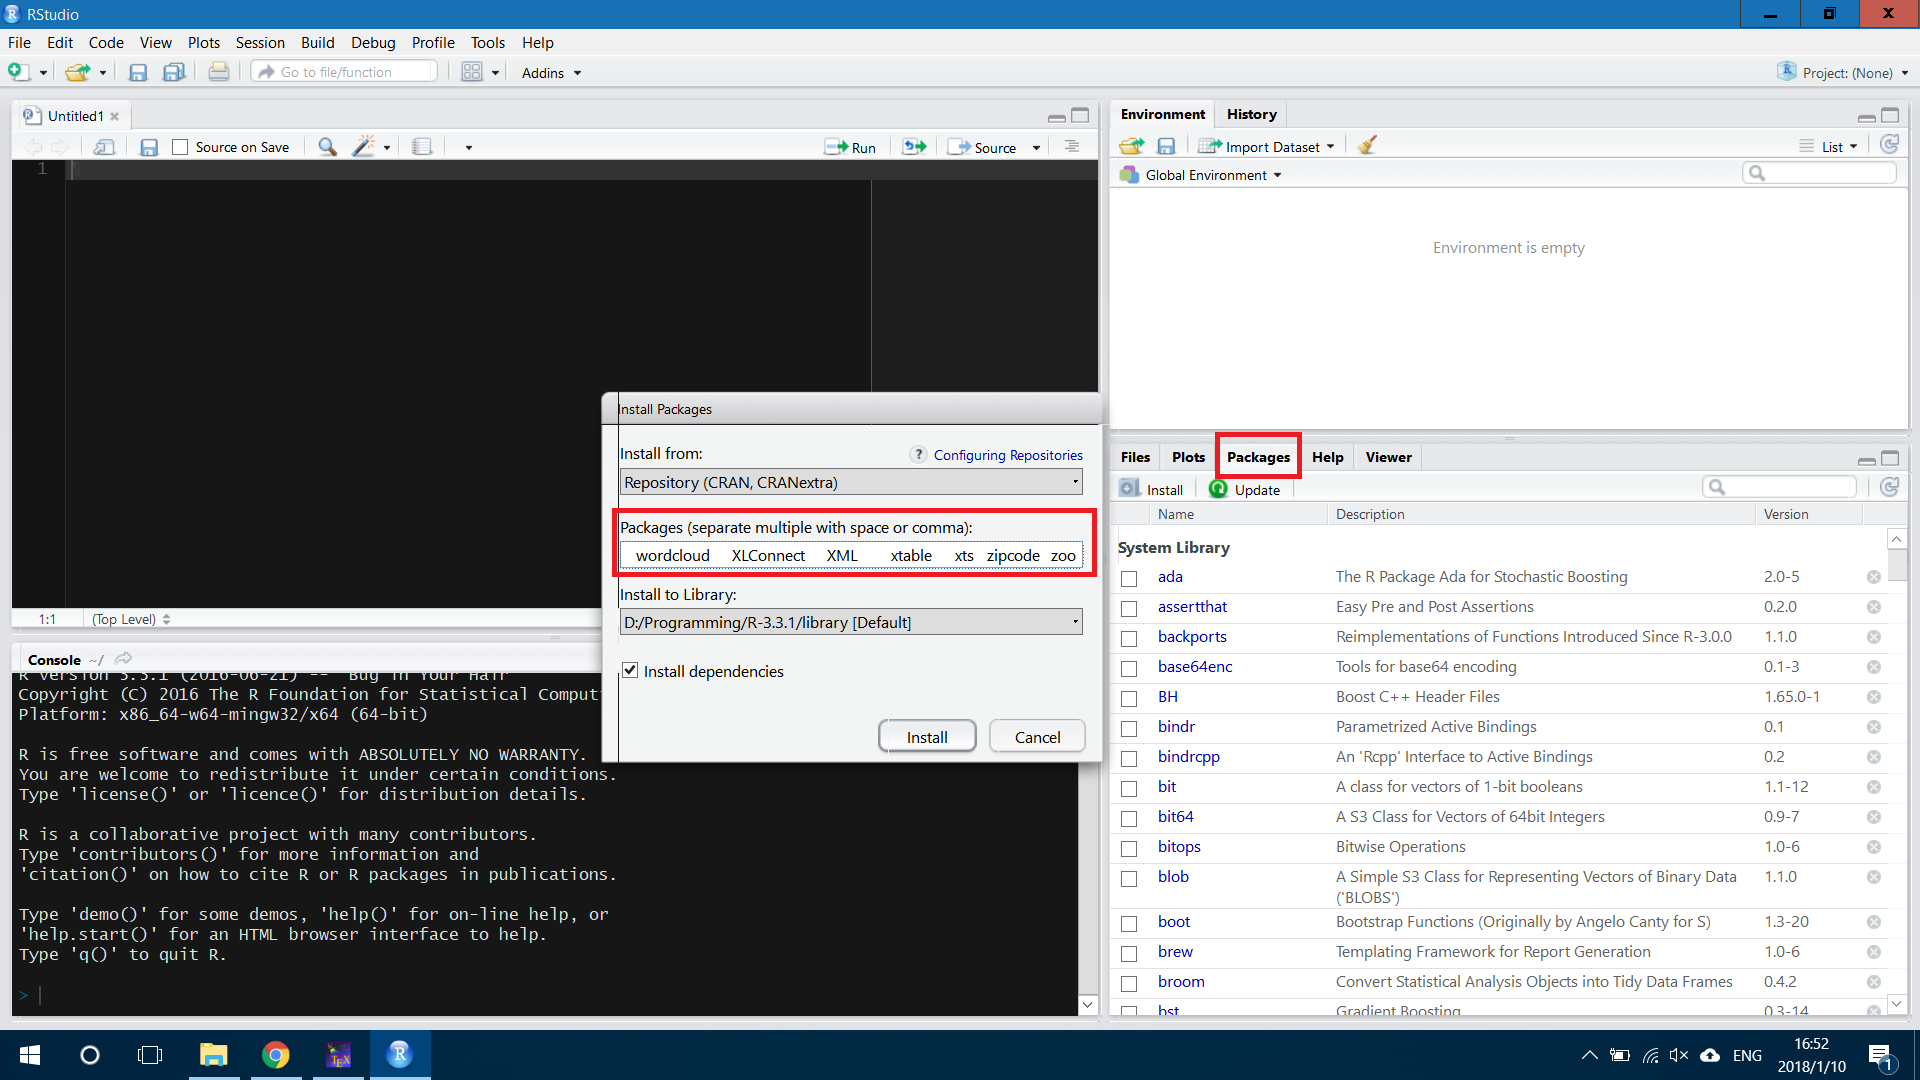
\includegraphics[width=0.7\linewidth]{figs/installPackages}
        \caption{}
        \label{fig:installpackages}
      \end{figure}

      To upgrade your packages, select all packages and press "Install Updates"

      \begin{figure}[h!]
        \centering
        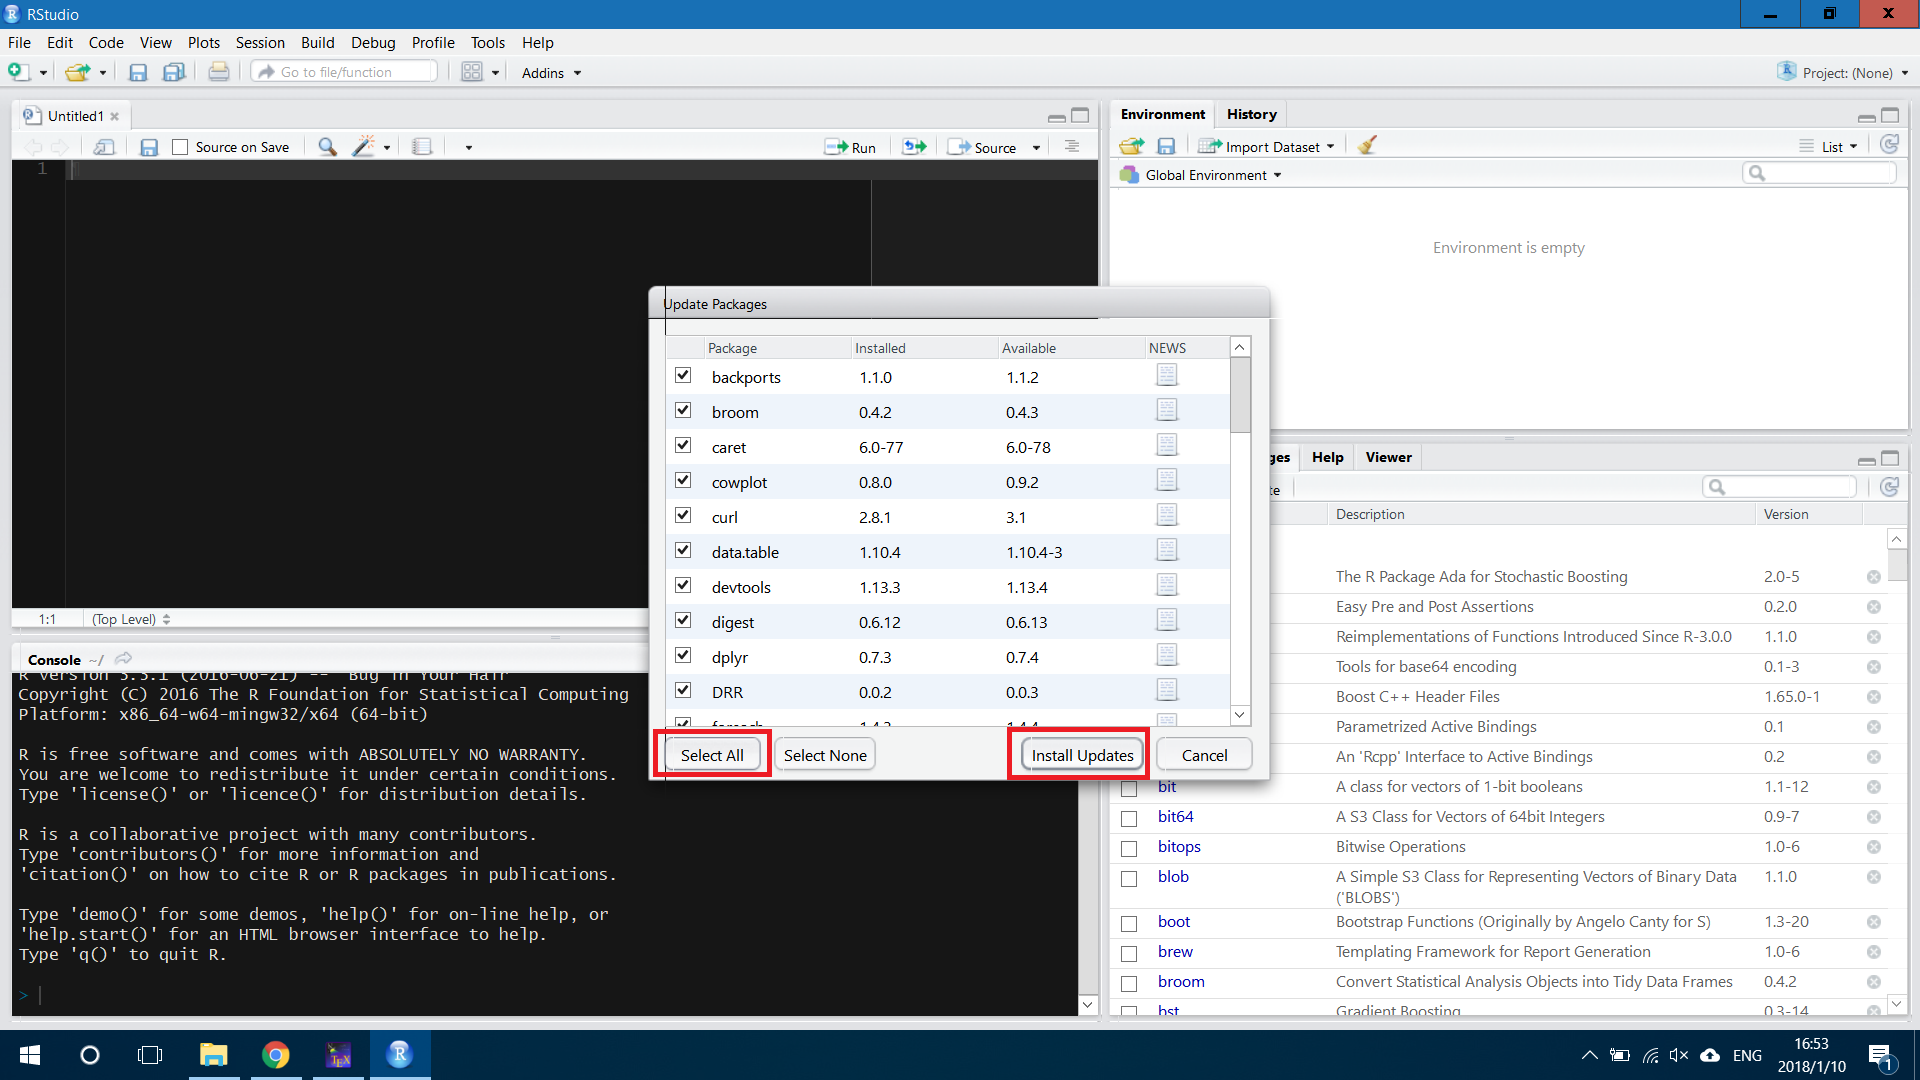
\includegraphics[width=0.7\linewidth]{figs/upgradePackages}
        \caption{}
        \label{fig:upgradepackages}
      \end{figure}

    \end{itemize}

Note that the ``R standard packages are listed under the ``For Windows'' section in subsubsection\ref{subsec:rstandpack}.  \\

  \subsection{For Windows}

  In Windows we are allowed to use spaces in filenames, however, most other systems does not support that.
  To avoid conflicts or troubles, we suggest using \href{https://sanaulla.info/2008/06/25/camelcase-notation-naming-convention-for-programming-languages/}{camelBack} naming convention or use "-" or "\_" to replace spaces.

    \subsubsection{LaTeX}

      \LaTeX~is a document preparation system that is widely used in the academia for producing scientific documents.
      You will need to install two softwares,  Miktex and TeXstudio. \\
      \begin{itemize}
        \item Download and run the Basic MiKTeX Installer.
        MiKTeX has the ability to install missing packages automatically, i.e., this installer is suitable for computers connected to the Internet.
        Before you run the installer, you can check the \href{https://miktex.org/kb/prerequisites-2-9}{prerequisites}.
        The installer is available on the \href{https://miktex.org/download}{download} page.
        You start it with a double-click on the downloaded file.
        \item Read the Copying Conditions carefully and click "I accept the MiKTeX copying conditions", the click "Next", as demonstrated below.

        \begin{figure}[!ht]
          \centering
          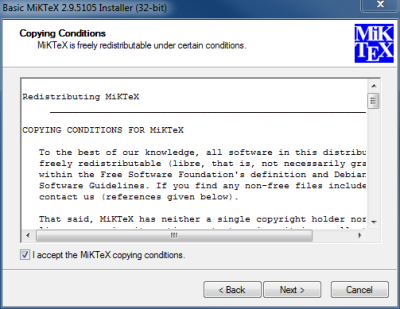
\includegraphics[width=0.7\linewidth]{figs/basic-miktex-license-2-9}
          \caption{}
          \label{fig:basic-miktex-license-2-9}
        \end{figure}
        \item You have the Option to create a shared MiKTeX installation.
        Click "Anyone who uses this Computer (all users), if you want to install MiKTeX for all users.
        Click "Only for ...", if you want to install MiKTeX for yourself only.
        When you have made your decision, click "Next" to go to the next page.

        \begin{figure}[h]
          \centering
          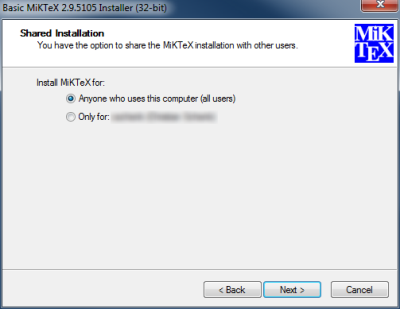
\includegraphics[width=0.7\linewidth]{figs/basic-miktex-shared-2-9}
          \caption{}
          \label{fig:basic-miktex-shared-2-9}
        \end{figure}

        \pagebreak

        \item You can specify the directory where you want to install your Miktex.
        Click "Browse", if you want to specify another (than the default) directory location.
        Click "Next", to go to the next page.

        \begin{figure}[!h]
          \centering
          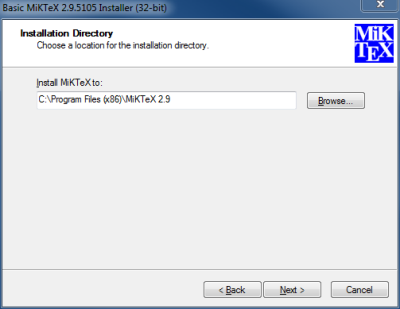
\includegraphics[width=0.7\linewidth]{figs/basic-miktex-installdir-2-9}
          \caption{}
          \label{fig:basic-miktex-installdir-2-9}
        \end{figure}
        \pagebreak
        \item The installer allows you to set the preferred paper size(usually it's A4 in China and letter size in the US).
        You also have the option to change the default behavior of the integrated package manager for the case where a required package is missing.
        Select "Yes", to make the package manager is always allowed to install missing packages.
        All these configurations can be changed later.

        Click "Next", to go to the next page.

        \begin{figure}[h!]
          \centering
          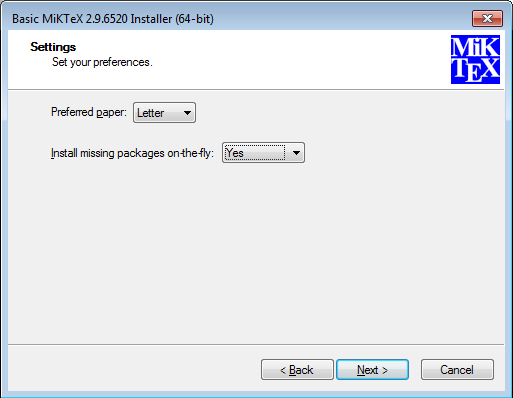
\includegraphics[width=0.7\linewidth]{figs/MikTex1.png}
          \caption{}
          \label{fig:basic-miktex-settings-2-9}
        \end{figure}
        \item Before the actual installation process begins, you get a chance to review your decisions.
        If you are satisfied with the settings, then click "Start" to start the actual installation.
        \item The installation will take a few minutes.
        The progress bar shows an approximate percentage of completion.
        When the installation has finished, you can click "Next" to open the last page.
        \item MiKTeX is now installed.
        Click "Close", to close the installer.
        \item In order to make use of latex the easiest way is to use a integrated development editor (IDE).
        \textbf{TeXstudio} is an free package that allows you to edit tex documents, compile and view them, it has syntax highlighting, auto completion, in line spell and grammar checker and much more.
        You can find the downloads page \href{https://www.texstudio.org/}{here} and click on \textbf{download now}.
        \item Once downloaded, run and start the installer.
        \item Accept all the default conditions, and start up TeXstudio to finish.
        \item If you need instructions on how to start using LaTeX, here are some \href{https://en.wikibooks.org/wiki/LaTeX}{tutorials}.
      \end{itemize}
      \pagebreak
    \subsubsection{Git}

      \textbf{Git Bash} is command line programs which allow you to interface with the underlying git program.
      Bash is a Linux-based command line, which has been ported over to Windows.
      \begin{itemize}
        \item  Download latest version of Git Bash on the \href{http://gitforwindows.org/}{official website}.
        \item Once Git Bash Windows installer is downloaded, run the executable file and follow the setups:
        \item Agree to the GNU General Public License and click "Next".
        \begin{figure}[h!]
          \centering
          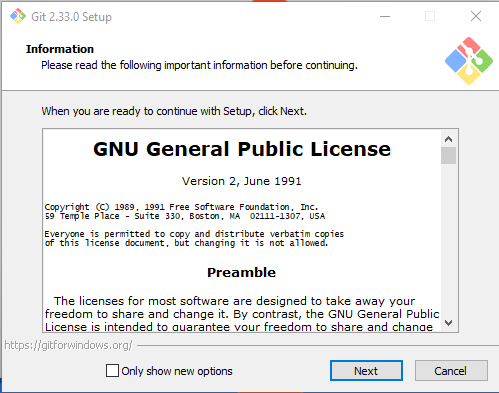
\includegraphics[width=0.58\linewidth]{figs/GitBash1}
          \caption{}
          \label{fig:gitbash1}
        \end{figure}

        \item Select the components you want to install and click Next.
        We suggest that you should unselect Windows Explorer integration.

        \begin{figure}[h!]
          \centering
          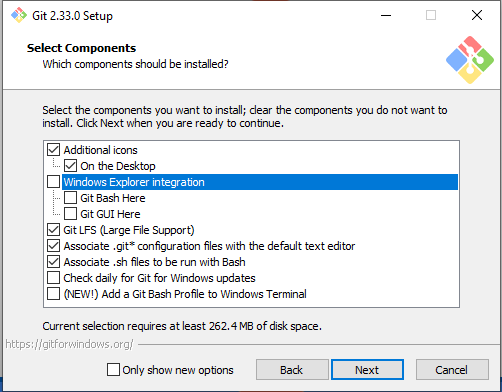
\includegraphics[width=0.55\linewidth]{figs/git2}
          \caption{}
          \label{fig:gitbash3}
        \end{figure}

    	\pagebreak

        \item Set default editor to Vim(which is the default option).

        \begin{figure}[h!]
          \centering
          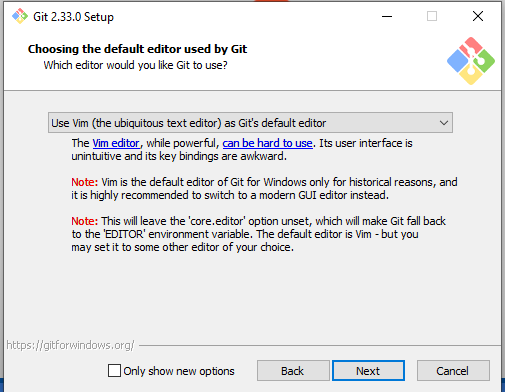
\includegraphics[width=0.65\linewidth]{figs/git1}
          \caption{}
          \label{fig:gitbash4}
        \end{figure}

    	\item Choose default initial branch name.

    	\begin{figure}[h!]
    		\centering
    		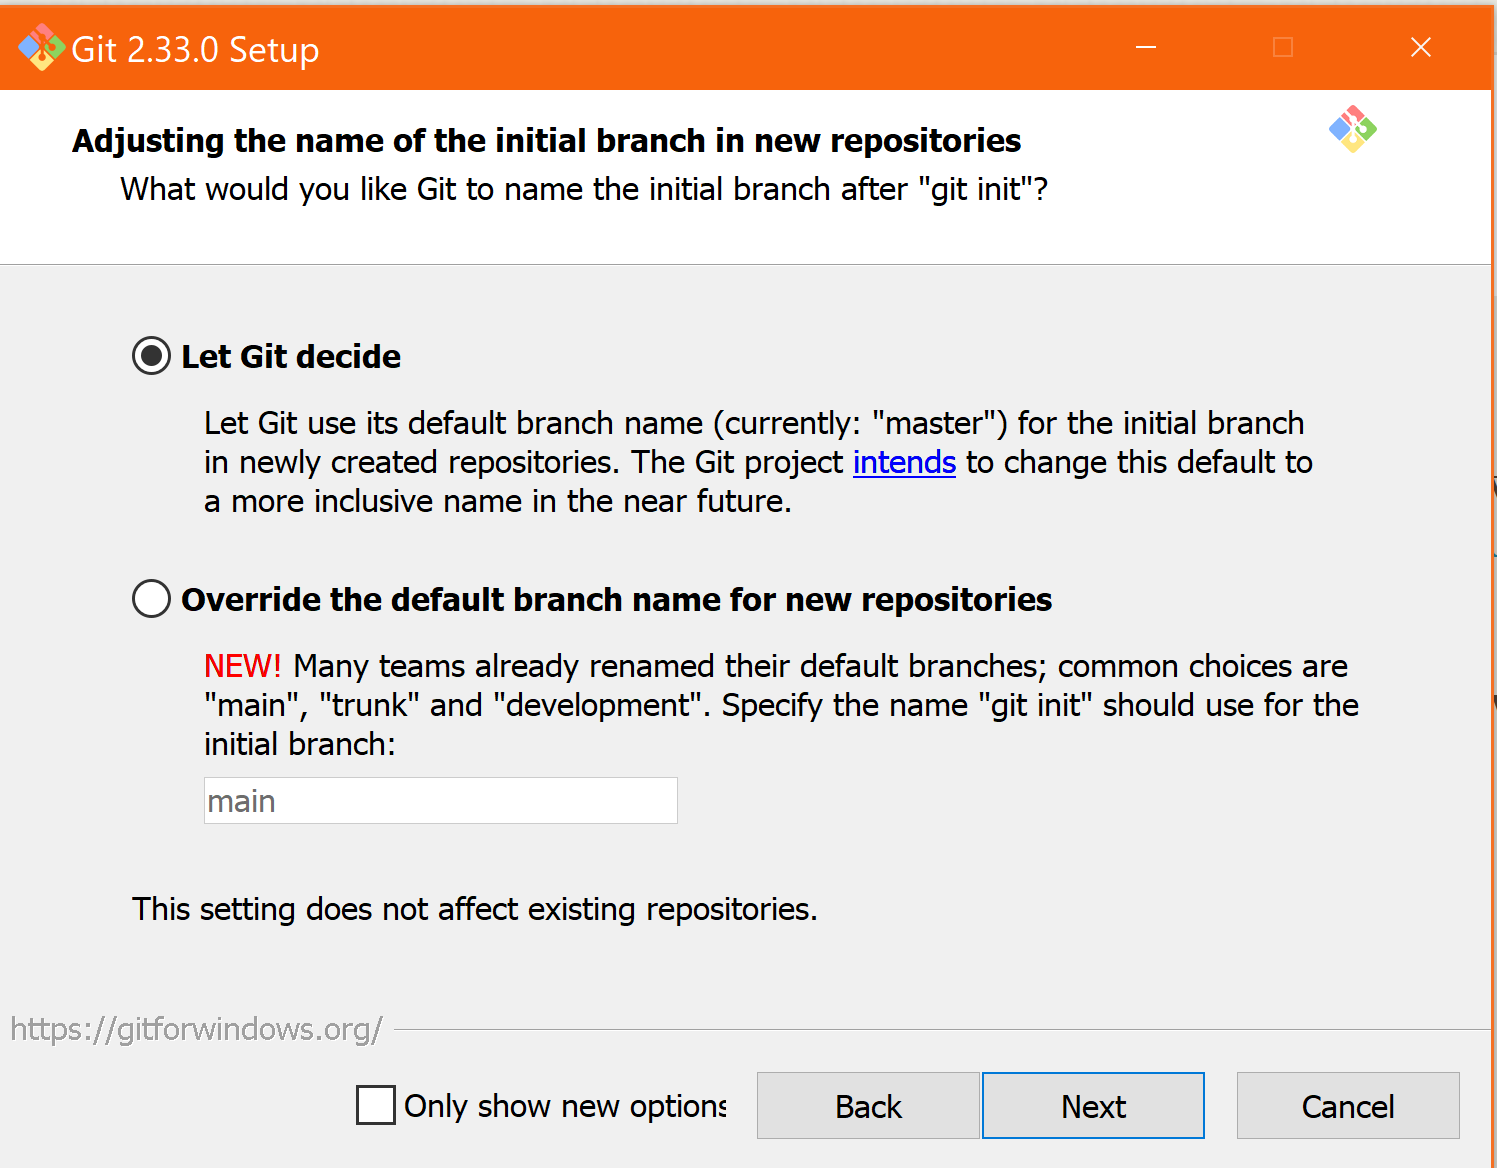
\includegraphics[width=0.7\linewidth]{figs/GitBash14_master}
    		\caption{}
    		\label{fig:gitbash14_master}
    	\end{figure}

    	\pagebreak

        \item We suggest that you use the default option, which is "Use Git from Git Bash only".

        \begin{figure}[h!]
          \centering
          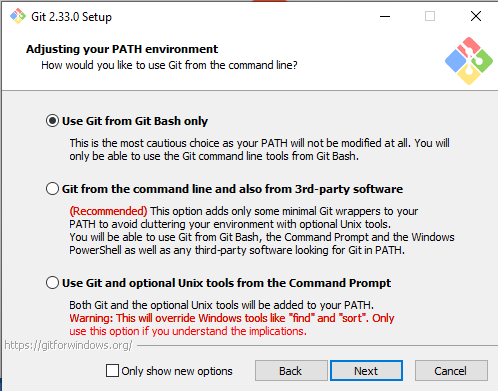
\includegraphics[width=0.7\linewidth]{figs/GitBash5}
          \caption{}
          \label{fig:gitbash5}
        \end{figure}

		\item Select which SSH client program to use.

		\begin{figure}[h!]
			\centering
			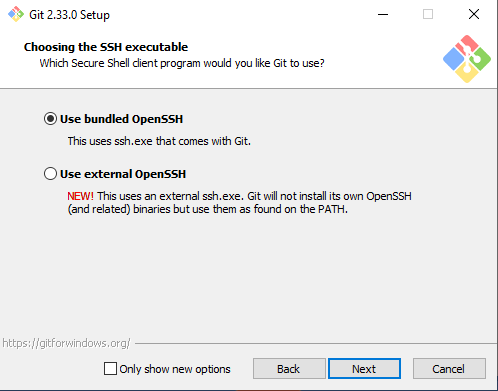
\includegraphics[width=0.7\linewidth]{figs/GitBash6}
			\caption{}
			\label{fig:gitbash6}
		\end{figure}

		\pagebreak

        \item Select which SSL/TLS library would you like to use for HTTPS connection and click Next.

        \begin{figure}[h!]
          \centering
          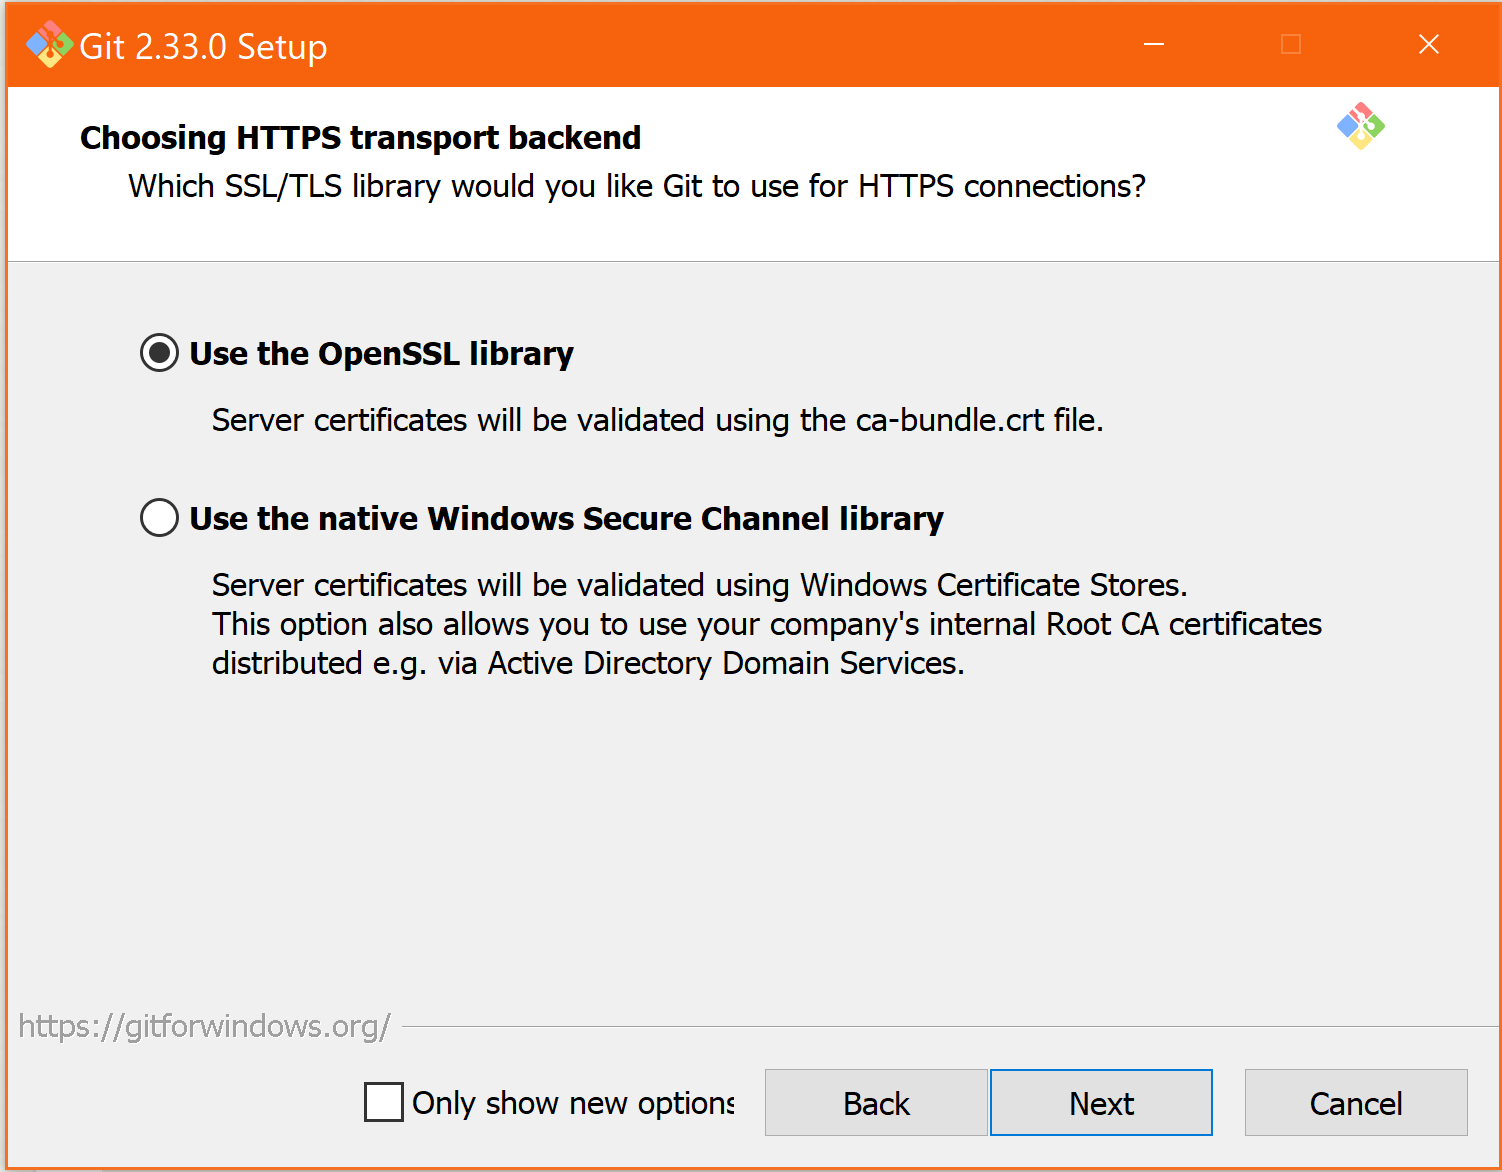
\includegraphics[width=0.7\linewidth]{figs/GitBash6b}
          \caption{}
          \label{fig:gitbash6b}
        \end{figure}

        \item Select, how should Git treat line endings in text files and click Next.

        \begin{figure}[h!]
          \centering
          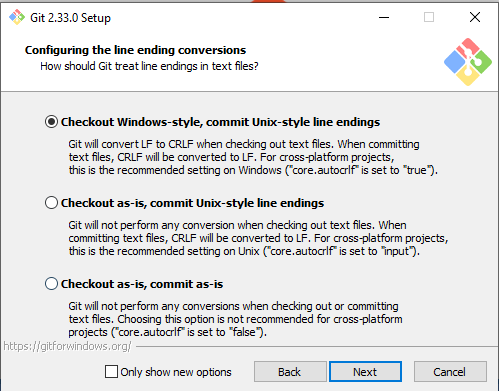
\includegraphics[width=0.7\linewidth]{figs/GitBash7}
          \caption{}
          \label{fig:gitbash7}
        \end{figure}

		\pagebreak

        \item Select the terminal you want to use for Git Bash.

        \begin{figure}[h!]
          \centering
          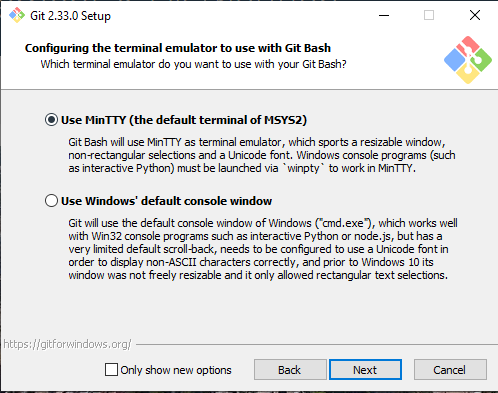
\includegraphics[width=0.7\linewidth]{figs/GitBash8}
          \caption{}
          \label{fig:gitbash8}
        \end{figure}

        \item Select the default behavior of 'git pull'

        \begin{figure}[h!]
        	\centering
        	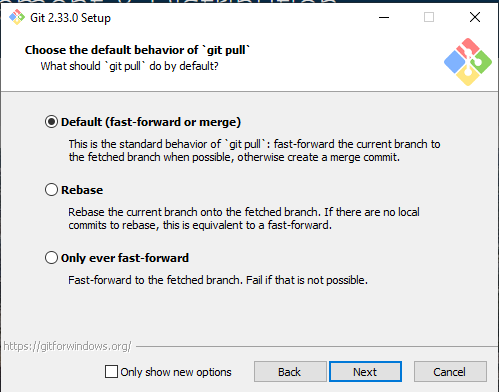
\includegraphics[width=0.7\linewidth]{figs/GitBash12}
        	\caption{}
        	\label{fig:gitbash12}
        \end{figure}

        \pagebreak

        \item Select the features you want to enable and click "Next".
        We suggest that you unselect "Enable Git Credential Manager".

        \begin{figure}[h!]
          \centering
          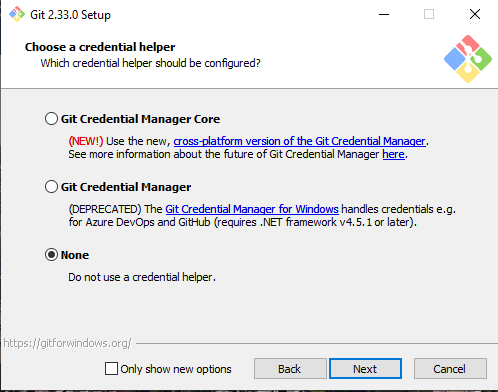
\includegraphics[width=0.7\linewidth]{figs/GitBash13}
          \caption{}
          \label{fig:gitbash13}
        \end{figure}

          \item Unselect the experimental options.

    \begin{figure}[h!]
    	\centering
    	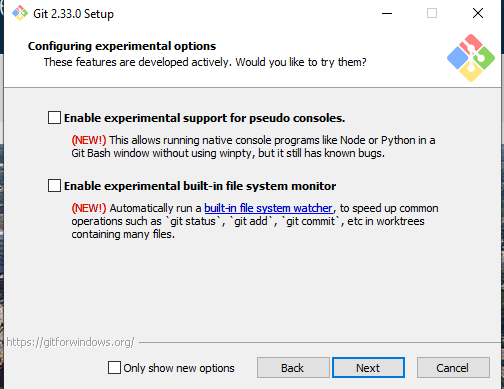
\includegraphics[width=0.7\linewidth]{figs/GitBash14}
    	\caption{}
    	\label{fig:gitbash14}
    \end{figure}

        \item Please wait while Setup wizard installs Git on your computer and click "Finish" to exit the Setup wizard.

        \item After Git Bash installation finishes you will ready to use the Linux command on a windows machine.
        Double click on below icon to start the Git Bash.

        \begin{figure}[h!]
          \centering
          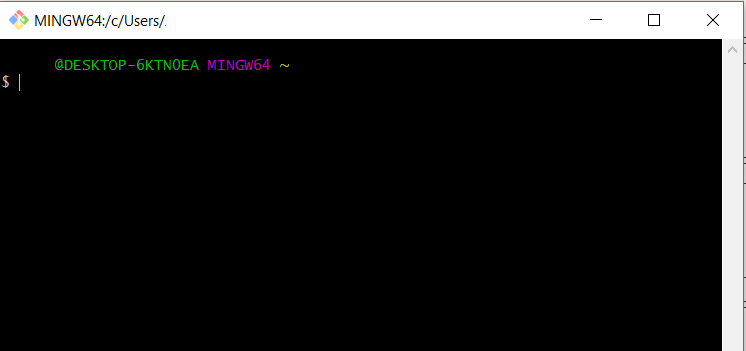
\includegraphics[width=0.7\linewidth]{figs/Launch-Git-Bash.png}
          \caption{}
          \label{fig:launchgitbash}
        \end{figure}

        \item Set up user name and email in Git.

        \begin{lstlisting}
        git config --global user.name "yourusername"
        git config --global user.email "youremail@website.com"
        git config --global color.ui auto
        \end{lstlisting}

        \item Here are some common commands you can use in git:
        \\
        \\
        pwd -- present working directory\\
        cd -- change directory\\
        ls -- list files in current working directory\\
        mkdir -- make new directory\\

        \item If you want to learn more about how git works (pull request, merge and more), you can read some \href{https://www.atlassian.com/git}{tutorials}.

      \end{itemize}

    \subsubsection{R}
      R is a free programming language and software environment for statistical computing and graphics that is supported by the R Foundation for Statistical Computing, while RStudio is a free and open-source integrated development environment for R.
      \begin{itemize}
        \item To \href{https://cran.r-project.org/}{download R}, please choose your "install R for Windows" and then choose base R for a complete installation.
        \item Double click on the installer, and follow the instructions.
        \item Users of Vista/Windows 7/8/Server 2008/2012 installing for a single user using an account with administrator rights should consider installing into a non-system area (such as C:\textbackslash R).
        \item Please try to avoid spaces or any special characters other than English letters and numbers in your installation directory, which may cause error later.
        \item After installing R, you can download \textbf{Rstudio} \href{https://www.rstudio.com/products/rstudio/download/}{here}, and choose the RStudio Desktop Open Source License version (the left most one).
        \item Run the installer and follow the installation instructions.
        \item Again, please try to avoid spaces or any special characters other than English letters and numbers in your installation directory.
        \item Rstudio have some built-in packages such as tidyverse and ggplot2, but if you are interested in building your own R packages, you can \href{https://cran.r-project.org/bin/windows/Rtools/}{download \textbf{Rtools}}.
        Please choose the latest version, as the older versions are not compatible with latest release of R.
        \item Run the installer, and accept the defaults throughout.
        \item Confirm and finish the installation.
        \item Once the Rtools installation completes, open RStudio and go to Profile--Global options--Code and change the code editing options as follows:

        \begin{figure}[h!]
          \centering
          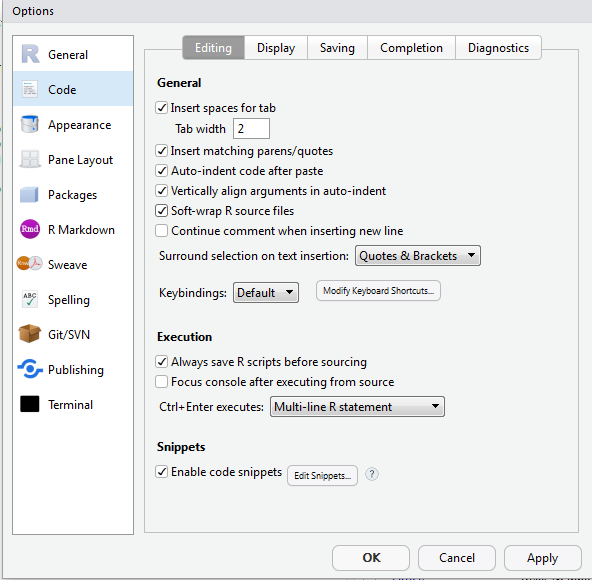
\includegraphics[width=0.6\linewidth]{figs/softwrapRsourcefile}
          \caption{}
          \label{fig:softwraprsourcefile}
        \end{figure}
        \pagebreak
        %	\item To install devtools, use
        %	\begin{lstlisting}
        %	install.packages("devtools")
        %	\end{lstlisting}
        \begin{figure}[h!]
          \centering
          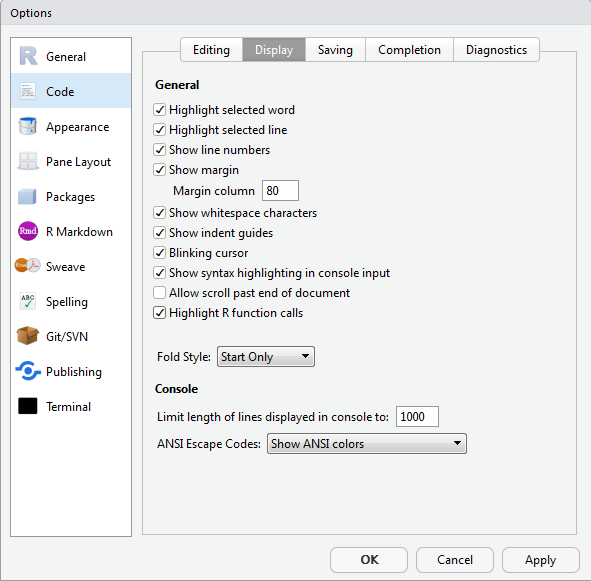
\includegraphics[width=0.6\linewidth]{figs/highlightRfunctioncall}
          \caption{}
          \label{fig:highlightrfunctioncall}
        \end{figure}
        \pagebreak
        \item You can also change your appearance style in Global Options:

        \begin{figure}[h!]
          \centering
          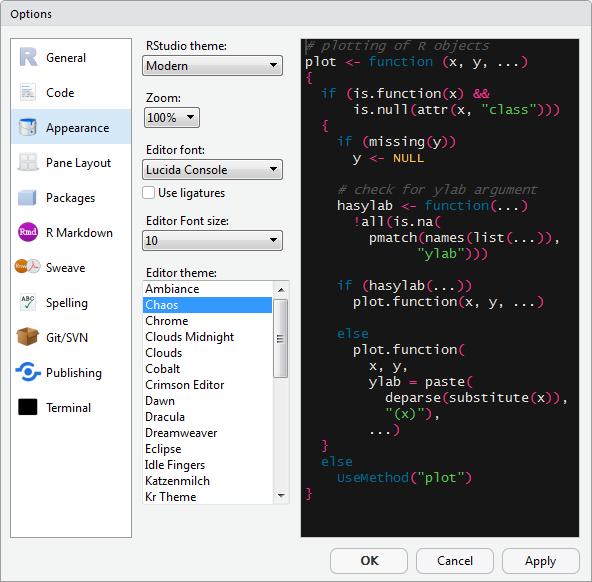
\includegraphics[width=0.6\linewidth]{figs/chaos}
          \caption{}
          \label{fig:chaos}
        \end{figure}
      \end{itemize}


    \subsubsection{GVim}

      GVim offers a graphic user interface for the editor \textbf{Vim}.
      This is a powerful editor but could be a little bit hard to use.
      \begin{itemize}
        \item You can download Vim from their \href{https://vim.sourceforge.io/download.php}{download page}.
        For Windows system, click on "\href{https://vim.sourceforge.io/download.php#pc}{PC: MS-DOS and MS-Windows}", and download "gvim80.exe".
        \item Open the installer and accept the default conditions.
      \end{itemize}

  \subsection{For Linux}

    \subsubsection{LaTeX}

      TeX Live is an easy way to get up and running with the TeX document production system, it is available on most Unix-like systems, but it is recommended to use MacTeX if you are using MacOSX.
      To install TeXLive and TeXstudio, run the following code:
      \begin{lstlisting}
      sudo apt-get install texlive-full texworks texstudio
      \end{lstlisting}
      \subsubsection{Git}
      To install Git, run the following code:
      \begin{lstlisting}
      sudo apt-get install git
      \end{lstlisting}

    \subsubsection{R}

      \begin{itemize}

        \item Install from CRAN:

        \begin{lstlisting}
        ## This sets up the CRAN repository in your Linux Package Manager
        sudo echo "deb http://cran.rstudio.com/bin/linux/ubuntu xenial/" |
        sudo tee -a /etc/apt/sources.list
        gpg --keyserver keyserver.ubuntu.com --recv-key E084DAB9
        gpg -a --export E084DAB9 | sudo apt-key add -
        sudo apt-get update
        sudo apt-get install r-base r-base-dev
        ## extra linux packages needed by
        sudo apt-get install r-cran-xml pkg-config libxml2-dev
        libtiff5-dev fftw3 fftw3-dev  tmux
        cifs-utils openssh-server openssh-client tree htop
        gdebi curl libcurl4-openssl-dev libssl-dev ffmpeg

        \end{lstlisting}

    	\pagebreak

    	\begin{figure}[h!]
    		\centering
    		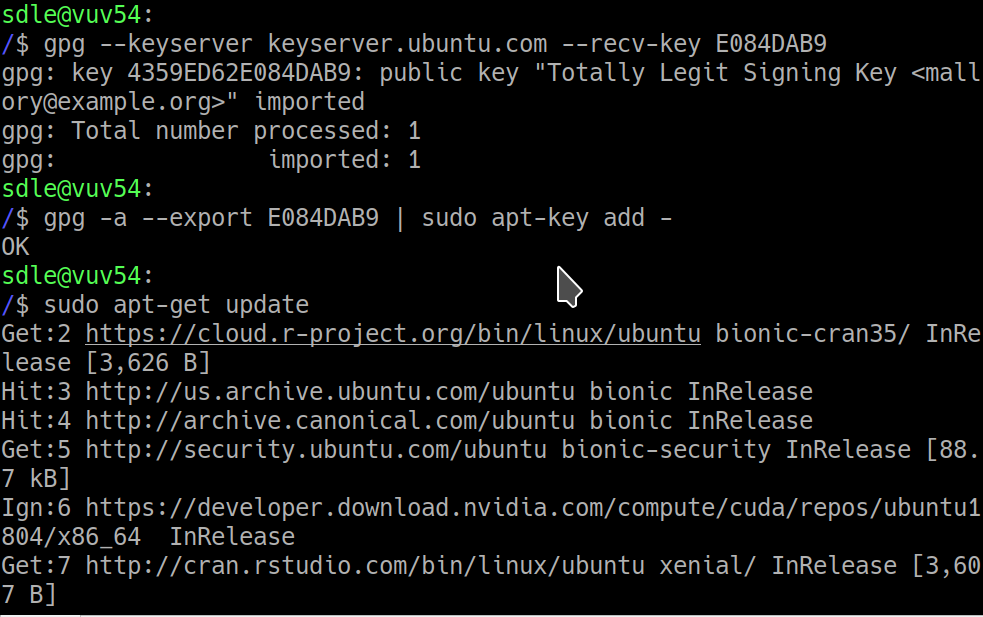
\includegraphics[width=0.7\linewidth]{figs/linux_r_install_gpgkeyserver}
    		\caption{}
    		\label{fig:linux_install_gdgpackages}
    	\end{figure}

        \begin{figure}[h!]
    		\centering
    		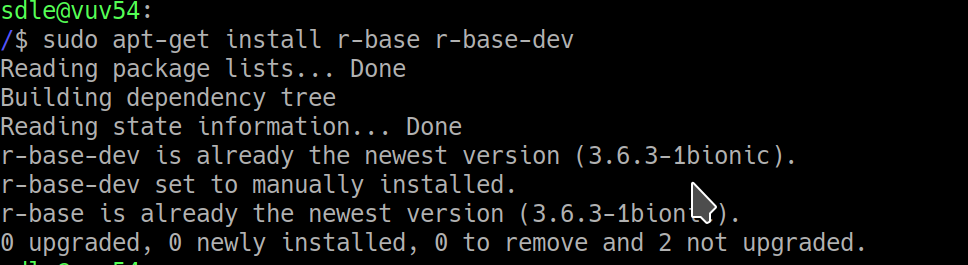
\includegraphics[width=0.7\linewidth]{figs/linux_r_install_r_base}
    		\caption{}
    		\label{fig:linux_install_base_r}
  		\end{figure}

    	\begin{figure}[h!]
    		\centering
    		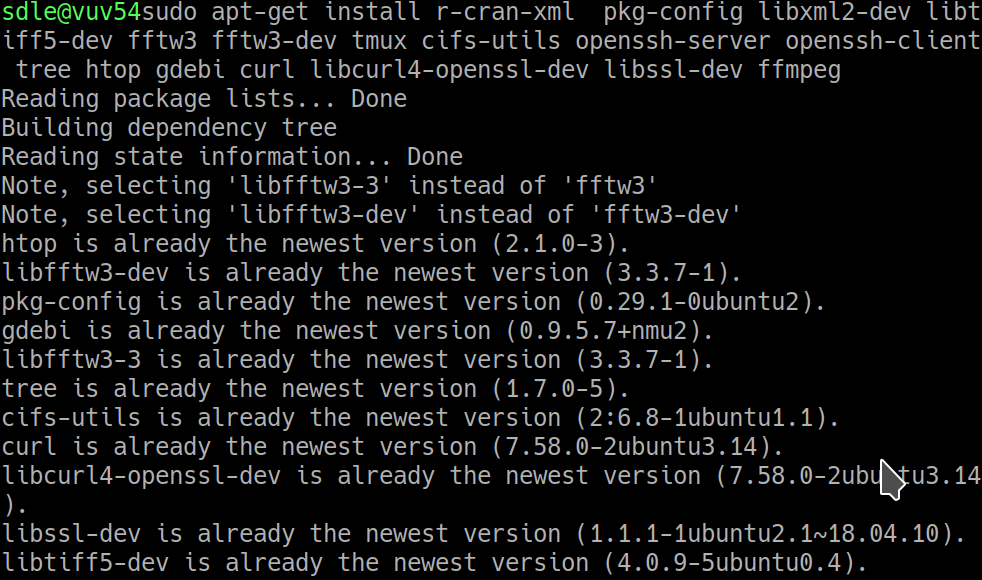
\includegraphics[width=0.7\linewidth]{figs/linux_r_install_packages}
    		\caption{}
    		\label{fig:linux_install_packages}
    	\end{figure}

    	\pagebreak

        \item Before installing, you should \href{https://www.rstudio.com/products/rstudio/download/}{check the latest version} of RStudio, and change the version number in the code below accordingly.
        Install RStudio:

        \begin{lstlisting}

        ## Update to the latest version number in the lines below
        wget https://download1.rstudio.org/rstudio-1.4.1717-amd64.deb
        sudo gdebi -n rstudio-1.4.1717-amd64.deb
        rm rstudio-1.4.1717-amd64.deb

        \end{lstlisting}

    	\begin{figure}[h!]
			\centering
			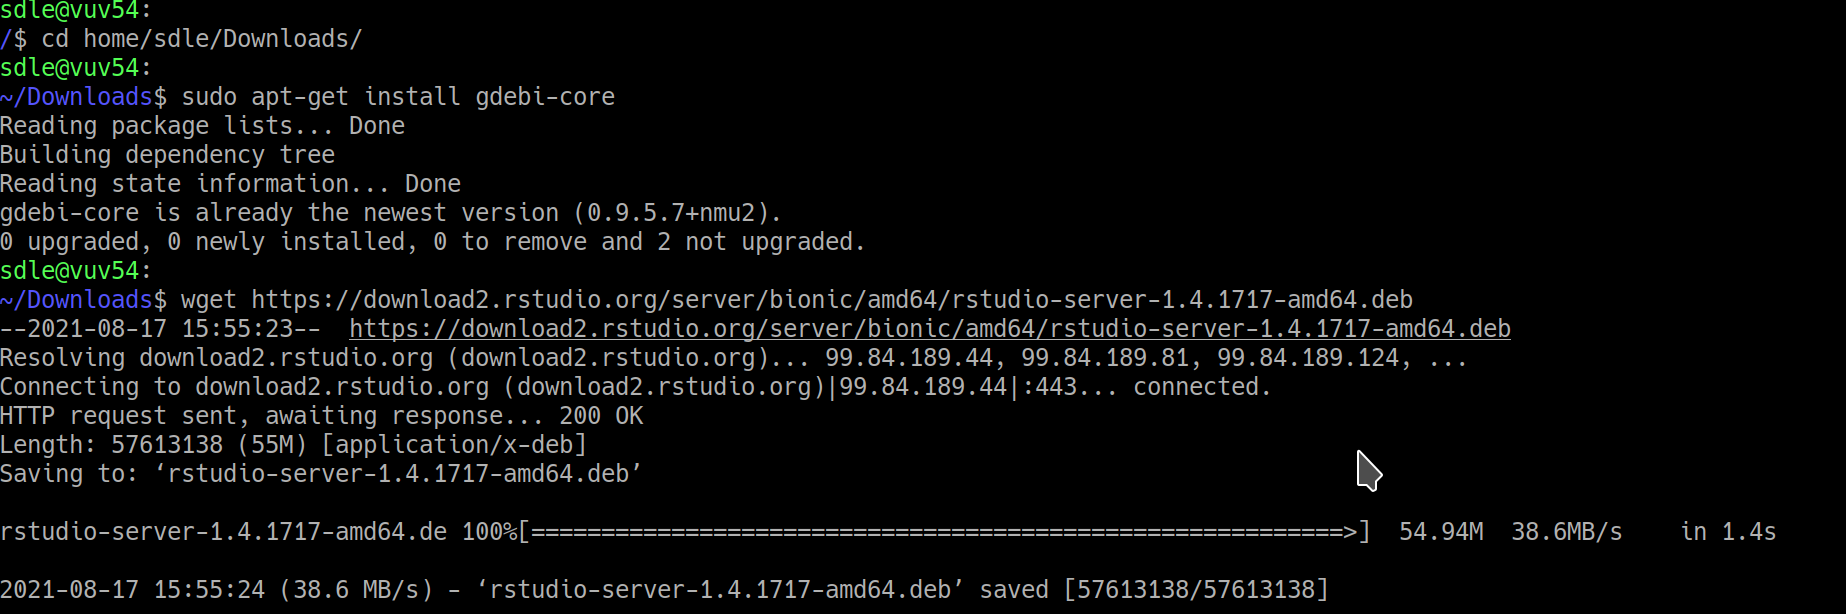
\includegraphics[width=0.7\linewidth]{figs/linux_r_install_rstudio_download}
			\caption{}
			\label{fig:linux_install_packages_rstudio_dl}
		\end{figure}

        \begin{figure}[h!]
        	\centering
        	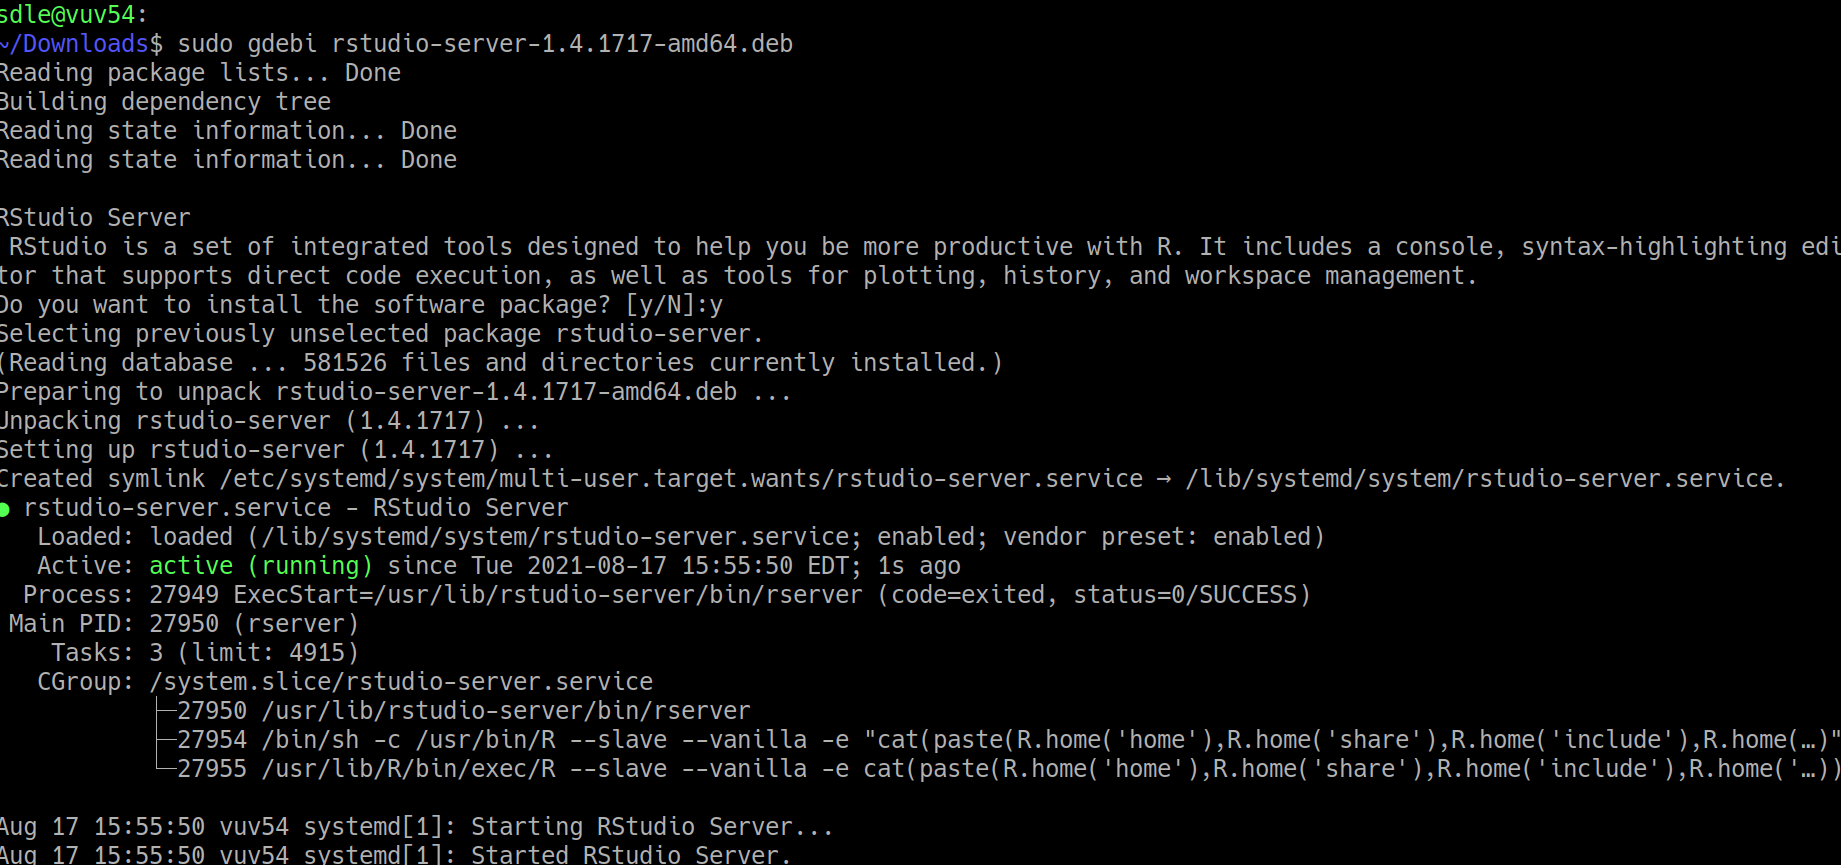
\includegraphics[width=0.7\linewidth]{figs/linux_r_install_rstudio_install}
        	\caption{}
        	\label{fig:linux_install_packages_rstudio_install}
        \end{figure}

      \item Once Rstudio is installed, Install the ``Standard R Packages'' listed here in Section \ref{subsec:rstandpack}.

      \end{itemize}

  \subsection{For Mac}

    \subsubsection{Homebrew}

      Homebrew is a package manager for Mac OS.
      To install Homebrew, paste and run the following command in terminal:
      \begin{lstlisting}
      /usr/bin/ruby -e "$(curl -fsSL https://raw.githubusercontent.com/Homebrew/
      install/master/install)"
      \end{lstlisting}
      You can read more about Homebrew \href{https://brew.sh/}{here}.

    \subsubsection{XQuartz}

      To correctly set up your linux environment, you should also install XQuartz.
      XQuartz is Apple Inc.'s version of the X server, a component of the X Window System for macOS.
      You can \href{https://www.xquartz.org/}{download} and install the latest version of XQuartz.

    \subsubsection{LaTeX}

      To install LaTeX on Mac, you need to install MacTeX and TeXstudio.
      \begin{itemize}
        \item The current distribution as of today (\today)is MacTeX-2017.
        This distribution requires Mac OS 10.10, Yosemite, or higher and runs on Intel processors.
        To download, click \href{http://www.tug.org/mactex/mactex-download.html}{MacTeX Download}.
        \item After downloading, double click on the MacTeX.pkg to install.
        Follow the straightforward instructions.
        Installation on a recent Macintosh takes four to six minutes.
        \item At the end of installation, the installer will report "Success." But sometimes, the installer puts up a dialog saying "Verifying..." and then the install hangs.
        In all cases known to us, rebooting the Macintosh fixes this problem.
        After the reboot, install again.
        \item Now you can start installing TeXstudio.
        You can find the corresponding installer on the \href{https://www.texstudio.org/}{TeXstudio website}.
        \item Because the developers of TeXstudio do not have an Apple Developer Account, OS X may complain about an unidentified developer and deny opening TXS.
        In that case, open the context menu on the TXS icon (Ctrl + Click) and select open.
      \end{itemize}

    \subsubsection{Git}

      There are several ways to install Git on a Mac.
      In fact, if you've installed XCode (or it's Command Line Tools), Git may already be installed.
      To find out, open a terminal and enter git --version.

      Apple actually maintain and ship their own fork of Git, but it tends to lag behind mainstream Git by several major versions.
      You may want to install a newer version of Git using the method below:
      \begin{itemize}
        \item Download the latest Git for \href{https://git-scm.com/download/mac}{Mac installer}.
        \item Follow the prompts to install Git.
        \item Open a terminal and verify the installation was successful by typing git --version.
        \item Configure your Git username and email using the following commands, replacing "yourusername" with your own.
        These details will be associated with any commits that you create:
        \begin{lstlisting}
        $ git config --global user.name "yourusername"
        $ git config --global user.email "youremail@website.com"
        \end{lstlisting}
      \end{itemize}

    \subsubsection{R}

      \begin{itemize}
        \item Download R from \href{http://cran.us.r-project.org/}{CRAN} and click "Download R for (Mac) OS X".
        \item Follow the instructions and install R.
        \item Download the latest RStudio from their \href{https://www.rstudio.com/products/rstudio/download/}{website}.
        Open the installer and follow the instructions.
        \item Once Rstudio is installed, Install the ``Standard R Packages'' listed here in Section\ref{subsubsec:rstandpack}.
      \end{itemize}

%-----------------------------------------

\bibliographystyle{ieeetr}
\bibliography{dsci351-451}

\end{document}
